\documentclass[11pt,a4paper]{article}
% Shared preamble for the mebi_plugin technical report.
% keep spaces inside \code (url drops them by default), and break there
\PassOptionsToPackage{obeyspaces,spaces}{url}
\usepackage[margin=2.3cm]{geometry}
\usepackage[T1]{fontenc}
\usepackage{lmodern}
\usepackage{microtype}
\usepackage{amsmath,amssymb,amsthm,mathtools}
\usepackage{mathpartir}
\usepackage{booktabs,longtable,tabularx,array}
\usepackage{xcolor}
\usepackage{listings}
\usepackage{tikz}
\usetikzlibrary{arrows.meta,positioning,shapes,fit,calc,automata,backgrounds}
\usepackage{enumitem}
\usepackage[numbers,sort&compress]{natbib}
\usepackage[hidelinks]{hyperref}
\usepackage{xurl}
\usepackage[nameinlink,capitalise]{cleveref}

\setlength{\parskip}{0.4em}
\setlength{\parindent}{0pt}
\setlength{\emergencystretch}{3em}
\setlist{nosep,leftmargin=*}

\theoremstyle{definition}
\newtheorem{definition}{Definition}[section]
\newtheorem{example}[definition]{Example}
\theoremstyle{plain}
\newtheorem{theorem}[definition]{Theorem}
\newtheorem{lemma}[definition]{Lemma}
\newtheorem{proposition}[definition]{Proposition}
\theoremstyle{remark}
\newtheorem*{remark}{Remark}

% ---- pointers into the code -------------------------------------------
% \loc{path}{line}      -> path:line         (one line)
% \locr{path}{from}{to} -> path:from--to     (a range)
% \file{path}           -> path              (a whole file)
% \code{text}           -> inline code (identifiers, commands)
% paths break at any character (xurl), so long ones do not overflow
\DeclareRobustCommand{\file}[1]{\nolinkurl{#1}}
\DeclareRobustCommand{\loc}[2]{\nolinkurl{#1:#2}}
\DeclareRobustCommand{\locr}[3]{\nolinkurl{#1:#2}\texttt{--#3}}
\DeclareRobustCommand{\code}[1]{\ifmmode\texttt{\detokenize{#1}}\else\nolinkurl{#1}\fi}

% ---- notation -----------------------------------------------------------
\newcommand{\tr}[1]{\xrightarrow{#1}}           % strong step
\newcommand{\wtr}[1]{\stackrel{#1}{\Longrightarrow}} % weak step
\newcommand{\silent}{\tau}
\newcommand{\Opt}{\mathsf{option}}
\newcommand{\Some}{\mathsf{Some}}
\newcommand{\None}{\mathsf{None}}
\newcommand{\wsim}{\precsim}                     % weak simulation
\newcommand{\wbis}{\approx}                      % weak bisimilarity
\newcommand{\pow}{\mathcal{P}}
\newcommand{\N}{\mathbb{N}}
\newcommand{\States}{\mathcal{S}}
\newcommand{\Labels}{\mathcal{A}}

% ---- listings -----------------------------------------------------------
\definecolor{kw}{RGB}{0,60,140}
\definecolor{cm}{RGB}{100,100,100}
\definecolor{bgc}{RGB}{247,247,247}
\lstdefinelanguage{Rocq}{
  morekeywords={Inductive,CoInductive,Definition,Fixpoint,CoFixpoint,Lemma,
    Theorem,Proof,Qed,Defined,Class,Instance,Section,End,Variable,Variables,
    Context,match,with,end,fun,forall,exists,let,in,if,then,else,Require,
    Import,From,Export,Module,Ltac,Record,Arguments,Hint,Set,Unset,Notation},
  sensitive=true,
  morecomment=[s]{(*}{*)},
  morestring=[b]",
}
\lstdefinelanguage{OCamlx}[Objective]{Caml}{morekeywords={;;}}
\lstset{
  basicstyle=\ttfamily\small,
  keywordstyle=\color{kw}\bfseries,
  commentstyle=\color{cm}\itshape,
  backgroundcolor=\color{bgc},
  frame=single, framerule=0pt,
  columns=fullflexible, keepspaces=true,
  breaklines=true, breakatwhitespace=true,
  showstringspaces=false,
  upquote=true,
  literate={→}{{$\to$}}1 {⇒}{{$\Rightarrow$}}1 {τ}{{$\tau$}}1 {≤}{{$\le$}}1
           {≥}{{$\ge$}}1 {×}{{$\times$}}1 {·}{{$\cdot$}}1 {—}{{---}}1 {–}{{--}}1
           {’}{{'}}1 {‘}{{`}}1,
}
\lstnewenvironment{rocq}[1][]{\lstset{language=Rocq,#1}}{}
\lstnewenvironment{ocaml}[1][]{\lstset{language=OCamlx,#1}}{}
\lstnewenvironment{shell}[1][]{\lstset{language={},#1}}{}

% ---- tikz styles -------------------------------------------------------
\tikzset{
  box/.style={draw,rounded corners=2pt,align=center,font=\small,inner sep=4pt},
  st/.style={circle,draw,minimum size=6mm,inner sep=1pt,font=\small},
  dep/.style={-{Stealth[length=2mm]}},
  lbl/.style={font=\scriptsize,fill=white,inner sep=1pt},
}


\title{\texttt{mebi\_plugin}: a technical report on its current state}
\author{The repository as of 10 November 2026\\ (Rocq 9.3.0, OCaml 5.4.1)}
\date{10 November 2026}

\begin{document}
\maketitle

\begin{abstract}
  \texttt{mebi\_plugin} (MEBI, \emph{Mechanised Bisimilarities}) is a
  Rocq plugin for strong and weak simulations and bisimilarities between
  states of labelled transition systems given as Rocq inductive
  predicates. A goal is decided by a symbolic engine on Sylvan's list
  decision diagrams, learned from the user's rules; Sylvan records each
  operation's result as it computes, and that log is the certificate. The
  plugin turns the log into lemma applications, a fact per operation,
  which Rocq's kernel typechecks: nothing is recomputed in Rocq. This
  report describes the engine, the reading of terms as containers that
  connects states to the diagrams' vectors, the certificate and its
  translation, the optimisations and how they fit the certificate, the
  commands, the tests and what remains. Each claim points at the code as
  \texttt{file:line}.
\end{abstract}

\tableofcontents
\clearpage

\section{Overview}\label{sec:overview}

\paragraph{What the plugin is for.} A \emph{labelled transition system}
(LTS) is a set of states and labelled steps between them. In Rocq, the
plugin takes an LTS as an inductive predicate
\code{step : M -> option A -> M -> Prop} without parameters: a step
\code{step s l s'} goes from \code{s} to \code{s'} with label \code{l}, and
the label \code{None} is a \emph{silent} step. Given two LTSs and a start
state in each, the plugin answers four kinds of goal
(\file{theories/Bisimilarity.v}): \code{strong_sim} and
\code{strong_bisimilar} (every step is answered by one step with the same
label), and \code{weak_sim} and \code{weak_bisimilar} (silent steps may be
taken freely around the answer). The tactics are \code{sim}, \code{bisim},
\code{weak_sim} and \code{weak_bisim}.

\paragraph{How a goal is decided and certified.} In three stages.
\begin{enumerate}
\item \textbf{Deciding} (\cref{sec:symbolic}). The engine reads the LTS's
  constructors as rules, reads each state as a \emph{container} (a shape,
  and a value at each position: \cref{sec:containers}), and stores sets of
  states as \emph{list decision diagrams} in Sylvan, a C library. It learns
  each rule's steps on the positions the rule reads, explores both systems,
  and plays the simulation game on pairs of states to its greatest
  fixpoint. The verdict is whether the start pair is in it.
\item \textbf{The certificate} (\cref{sec:prooflog}). The engine
  checks the game's result once more, as images, with Sylvan's \emph{proof log} on: every move from
  the relation found lands among the pairs that can answer it. Every
  result Sylvan computes (a union, a difference, an image) is recorded
  with the case its algorithm took. That log, kept in memory (or in a file
  next to the file being checked, on request), is the certificate: what
  Sylvan computed, step by step.
\item \textbf{The proof} (\cref{sec:prooflog:facts}, \cref{sec:qed}). The
  plugin turns each record into a \emph{fact}: a lemma of
  \file{theories/DdTree.v} applied to the record's nodes. From the facts
  and from proofs generated for the goal's own systems (each state as a
  vector, each learned step a real step, every real step learned), it
  builds the proof: its pieces as constants the kernel checks as they are
  made, and one term that names them, with which the tactic closes the
  goal. Rocq's kernel checks that term at \code{Qed}: it typechecks it.
  For a large goal, the command \code{MeBi Prove} builds the same proof
  with every part of it a constant, each checked as it is declared, and
  declares the lemma (\cref{sec:qed:prove}): it needs less memory.
\end{enumerate}

\paragraph{Reading path.} For a newcomer: \cref{sec:prooflog} first (it
defines every term it uses, with worked examples), then \cref{sec:qed}
for how the goal's proof is built from the certificate (it defines what
it needs from Rocq and recalls the terms of \cref{sec:prooflog}), then
\cref{sec:symbolic} for the engine and \cref{sec:containers} for the
encoding of states, then \cref{sec:optimisations} for how the
optimisations fit the certificate, and \cref{sec:commands,sec:tests} to
run things.

\section{The symbolic engine}\label{sec:symbolic}
\begingroup\sloppy

\providecommand{\Reach}{\mathit{Reach}}
\providecommand{\Uni}{U}
\providecommand{\pre}{\mathrm{pre}}
\providecommand{\post}{\mathrm{post}}
\providecommand{\Bad}{\mathit{Bad}}
\providecommand{\Ok}{\mathit{Ok}}
\providecommand{\lddsem}[1]{[\![#1]\!]}

This section describes the engine that decides every goal:
\code{strong_sim}, \code{strong_bisimilar}, \code{weak_sim} and
\code{weak_bisimilar} between closed start terms, without building an
explicit graph of the systems. It reads the user's LTS as a set of rules,
splits each state into a finite \emph{shape} and a vector of \emph{slot}
values, learns one transition relation per \emph{summand} (a rule chain) on
only the slots it reads, stores sets and relations as
Sylvan's~\cite{vandijk-vdpol15} List Decision Diagrams
(LDDs)~\cite{blom-vdpol08}, and decides the weak or the strong game as a
greatest fixpoint over pairs. With the log on, the game's last check is
repeated with Sylvan's proof log open: that log is the certificate
(\cref{sec:prooflog}). The engine is not trusted; the kernel checks the
certificate.

\paragraph{How a user reaches it.}
\begin{itemize}
\item The tactics \code{sim}, \code{bisim} (strong) and \code{weak_sim},
  \code{weak_bisim} (weak) (\file{src/g_mebi.mlg}) all call
  \code{Learn.check ~strong:(not weak)} (\file{src/user_tactics.ml},
  \code{read_goal}). With the prefix \code{debug} they also print
  \code{Learn.pr} (\cref{sec:sym-debug}).
\item \code{Print MeBi Rules <lts>} and
  \code{Print MeBi Skeleton <term> Using <lts>} (\file{src/g_mebi.mlg})
  print the first two stages.
\end{itemize}

\subsection{Map of the code}

\begin{center}
\small
\begin{tabularx}{\linewidth}{@{}l r >{\raggedright\arraybackslash}X@{}}
\toprule
File & lines & Role \\
\midrule
\file{lib/rules/rules.ml}, \file{.mli} & 209, 73 &
  An LTS's constructors read as rules (\cref{sec:sym-rules}). \\
\file{lib/skeleton/skeleton.ml}, \file{.mli} & 786, 138 &
  Structural constructors, shapes and slots, summands
  (\cref{sec:sym-skeleton}). \\
\file{lib/ldd/ldd.ml}, \file{.mli} & 123, 96 &
  OCaml interface to Sylvan's LDDs (\cref{sec:sym-ldd}). \\
\file{lib/ldd/ldd_stubs.c} & 235 & The C stubs. \\
\file{lib/ldd/dune} & 48 & Compiles Sylvan and Lace into the binding's
  library. \\
\file{vendor/sylvan/}, \file{vendor/lace/} & (C) & git submodules
  (forks): Sylvan on the branch \code{proof-log} (the proof log), Lace
  1.10.0 (\file{lib/ldd/README.md}). \\
\file{lib/learn/learn.ml}, \file{.mli} & 1195, 79 &
  The interpreter, learning, exploration, the game, the logged last check
  (\cref{sec:sym-learn,sec:sym-game,sec:sym-check}). \\
\file{test/ldd_tests.ml} & & 25 checks of the binding and the proof
  log, no Rocq; run in CI (\cref{sec:tests}). \\
\file{src/user_tactics.ml} & & \code{prove}: the four tactics, the call to
  \code{Learn.check}, the log's place; \code{check_log}. \\
\bottomrule
\end{tabularx}
\end{center}

The libraries depend on each other in a line:
\code{rocq-mebi.rules} $\leftarrow$ \code{rocq-mebi.skeleton}
$\leftarrow$ \code{rocq-mebi.learn} $\rightarrow$ \code{rocq-mebi.ldd}
(\file{lib/learn/dune}, \file{lib/skeleton/dune}). Only \code{ldd} is free
of \code{rocq-runtime}, which is why its test binary needs no Rocq.

\begin{figure}[t]
\centering
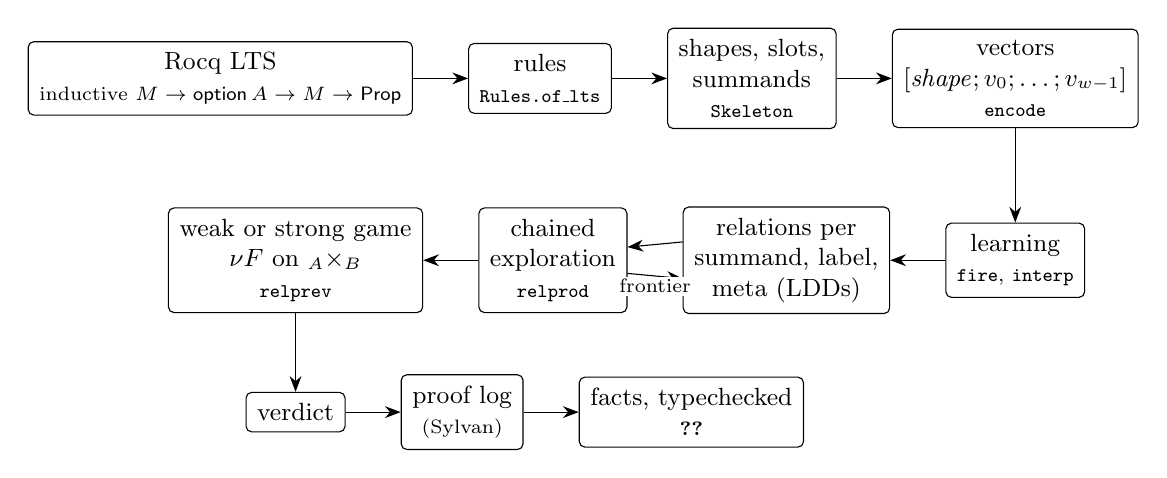
\begin{tikzpicture}[node distance=6mm and 7mm]
  \node[box] (lts) {Rocq LTS\\ \scriptsize inductive $M\to\Opt\,A\to M\to\mathsf{Prop}$};
  \node[box,right=of lts] (rules) {rules\\ \scriptsize \texttt{Rules.of\_lts}};
  \node[box,right=of rules] (skel) {shapes, slots,\\ summands\\ \scriptsize \texttt{Skeleton}};
  \node[box,right=of skel] (enc) {vectors\\ $[\mathit{shape};v_0;\dots;v_{w-1}]$\\ \scriptsize \texttt{encode}};
  \node[box,below=12mm of enc] (learn) {learning\\ \scriptsize \texttt{fire}, \texttt{interp}};
  \node[box,left=of learn] (rel) {relations per\\ summand, label,\\ meta (LDDs)};
  \node[box,left=of rel] (expl) {chained\\ exploration\\ \scriptsize \texttt{relprod}};
  \node[box,left=of expl] (game) {weak or strong game\\ $\nu F$ on $\Reach_A\times\Reach_B$\\ \scriptsize \texttt{relprev}};
  \node[box,below=10mm of game] (verdict) {verdict};
  \node[box,right=of verdict] (cert) {proof log\\ \scriptsize (Sylvan)};
  \node[box,right=of cert] (coq) {facts, typechecked\\ \scriptsize \cref{sec:prooflog}};
  \draw[dep] (lts) -- (rules);
  \draw[dep] (rules) -- (skel);
  \draw[dep] (skel) -- (enc);
  \draw[dep] (enc) -- (learn);
  \draw[dep] (learn) -- (rel);
  \draw[dep] (rel.170) -- (expl.10);
  \draw[dep] (expl.-10) -- node[lbl,below]{frontier} (rel.-170);
  \draw[dep] (expl) -- (game);
  \draw[dep] (game) -- (verdict);
  \draw[dep] (verdict) -- (cert);
  \draw[dep] (cert) -- (coq);
\end{tikzpicture}
\caption{The symbolic pipeline, and the certificate it leaves.}
\label{fig:sym-pipeline}
\end{figure}

\subsection{Rules: \texttt{lib/rules}}\label{sec:sym-rules}

\begin{definition}[Rule]
Let \code{L : M -> option A -> M -> Prop} be an inductive without
parameters (checked by \code{Rocq_utils.lts_shaped}). Each constructor
\[
  c : \forall\, x_1\dots x_k,\ P_1 \to \dots \to P_m \to L\ s\ \ell\ t
\]
is a rule $\rho_c$ with variables $\vec x$ (the binders that are not
propositions), premises $P_1,\dots,P_m$ (the binders that are), source
$s$, label $\ell$ and target $t$. A premise is
\begin{itemize}
\item \code{Step}: a step $L'\ s'\ \ell'\ t'$ of an LTS $L'$ (any LTS, not
  necessarily $L$);
\item \code{Decide}: a proposition $P$ for which typeclass resolution finds
  an instance of stdlib's \code{Decidable P}; the rule keeps
  \code{Decidable_witness P i}, a boolean over the rule's variables;
\item \code{Opaque}: any other proposition (an equation, \code{In}, a
  relation, an existential).
\end{itemize}
\end{definition}

The types are at \locr{lib/rules/rules.mli}{15}{51}. Every term of a rule
is over the \emph{whole} context \code{ctx} in de Bruijn indices: each
premise, read in the context of the binders before it, is lifted over the
rest (\loc{lib/rules/rules.ml}{108}). \code{rule}
(\locr{lib/rules/rules.ml}{87}{139}) classifies each binder: a non-\code{Prop}
binder is a variable (\loc{lib/rules/rules.ml}{110}); a \code{Prop} binder
is a \code{Step} if its head is an LTS-shaped inductive applied to three
arguments (\code{step_args}, \locr{lib/rules/rules.ml}{68}{78}), else a
\code{Decide} if \code{witness} (\locr{lib/rules/rules.ml}{50}{63}) finds a
\code{Decidable} instance, else \code{Opaque}
(\loc{lib/rules/rules.ml}{122}). The conclusion must be a step of the
same inductive, or \code{Not_an_lts} is raised. \code{of_lts}
(\locr{lib/rules/rules.ml}{142}{166}) returns the rules of the root LTS
and, transitively, of every LTS its \code{Step} premises use, first met
first. The \code{Decidable} class must be loaded:
\file{theories/loader.v} \code{Require}s (does not import)
\code{Stdlib.Classes.DecidableClass}.

\code{Opaque} premises are kept; the interpreter
stops at them (\cref{sec:sym-interp}) and the skeleton marks the summand
dynamic.

\begin{example}[\code{Print MeBi Rules}]
\begin{rocq}
Inductive step : tm -> option act -> tm -> Prop :=
| s_pre x k : step (pre x k) (Some x) k
| s_hide k l k' : step k l k' -> visible l = true -> step (hide k) l (hide k').
\end{rocq}
reads as two rules; \code{s_hide} has a \code{Step} premise and a
\code{Decide} premise (\code{=} on \code{bool} has a stdlib instance). The
rule \code{q : forall n m, (exists k, k = n) -> opaque n None m} has an
\code{Opaque} premise, printed with \code{[Opaque]}
(\loc{lib/rules/rules.ml}{180}).
\end{example}

\paragraph{Stale comments.} \file{lib/rules/dune} says ``only the plugin
(src/) uses it'' and ``S3's bit format goes in a library of its own'';
\file{doc/s2-linearisation.md} decision 8 says the same. Today
\file{lib/skeleton}, \file{lib/learn} and \file{lib/certify} use it, and
the bit format is gone.

\subsection{The skeleton: \texttt{lib/skeleton}}\label{sec:sym-skeleton}

Phase~1 turns a start term into a vector whose positions a rule touches
locally. Everything is computed from the user's rules, with no knowledge
of any calculus (\file{doc/skeleton.md}).

\subsubsection{Structural constructors}

\begin{definition}[Structural]
For a rule $\rho$ with source $s$ and target $t$, a constructor $c$
occurring in $s$ at path $\pi$ (a list of field indices, parameters
excluded) is \emph{kept} by $\rho$ if $t$ has a constructor application
with head $c$ at the same path $\pi$. $c$ is \emph{structural} for $L$ if
some rule of $L$ keeps it. Constructors that occur in sources but that no
rule keeps are \emph{never kept}.
\end{definition}

\code{classify} (\locr{lib/skeleton/skeleton.ml}{103}{125}) computes both
lists from \code{occurrences} and \code{at}
(\locr{lib/skeleton/skeleton.ml}{81}{96}). Only the rules of the root LTS
are used (\code{structural_of}, \locr{lib/skeleton/skeleton.ml}{726}{733}).
CCS's \code{par} is structural (kept by \code{s_parl}); Proc's \code{cpar}
is structural although \code{do_par_end} dissolves it, since
\code{do_parl} keeps it. \code{pre}, \code{tend} are never kept.

An earlier version (same day) took the constructors that \emph{every} rule
keeps and collapsed a node into one slot where a rule changed its shape.
Proc then had no skeleton at all, so the shape became part of the state
instead (decision D3 of \file{SYMBOLIC_PLAN.md}).

\subsubsection{Shapes, slots and the canonical split}

\begin{definition}[Shape, split]
A \emph{shape} is a tree $\sigma ::= \mathsf{Slot}\ i \mid
\mathsf{Node}(c, \vec p, \sigma_1\dots\sigma_n)$ with $c$ structural and
$\vec p$ its type parameters (\locr{lib/skeleton/skeleton.ml}{5}{14}).
The \emph{canonical split} of a closed term $t$ is
\[
\mathrm{split}(t) =
\begin{cases}
\mathsf{Node}(c,\vec p,\mathrm{split}(t_1)\dots\mathrm{split}(t_n)) &
  t = c\ \vec p\ t_1\dots t_n \text{ fully applied},\ c \text{ structural}\\
\mathsf{Slot}\ i,\ \text{with value } t & \text{otherwise}
\end{cases}
\]
slots numbered $0,1,\dots$ left to right (\code{split},
\locr{lib/skeleton/skeleton.ml}{736}{753}; inverse \code{rebuild},
\locr{lib/skeleton/skeleton.ml}{756}{765}). A slot's value never starts
with a structural constructor. Shapes are compared by \code{key}
(\locr{lib/skeleton/skeleton.ml}{134}{142}), a string of the structure
with slots unnumbered.
\end{definition}

A \emph{state} is a shape together with its slot values. Since a slot
value is never structural, a rule's structural constructors match nodes
only, and every other part of its source reads slot values.

\paragraph{A possible key collision.} \code{key} prints a constructor as
its mutual block's name and the constructor's index
(\code{MutInd.to_string (fst (fst n.cons))}, \code{snd n.cons}); it omits
the index of the inductive within the block, and the parameters. Two
structural constructors with the same index in two inductives of one
mutual block, or one polymorphic constructor at two parameter
instantiations, would get the same key. No example in the repository has
either; it is a latent issue, not an observed one.

\subsubsection{Summands}

\begin{definition}[Summand, origins]
A \emph{summand} of a shape $\sigma$ (\locr{lib/skeleton/skeleton.ml}{31}{37})
is a rule chain that can fire from $\sigma$: a list of rule names,
outermost first, where \code{<L>} stands for ``a step of a closed value by
$L$, computed at run time''; the source slots it \emph{reads}; its
\emph{target} $\tau ::= \mathsf{TSlot}(o) \mid \mathsf{TNode}(c,\vec
p,\tau_1\dots\tau_n)$ with origins $o ::= \mathsf{Moved}\ i \mid
\mathsf{Computed}\ \vec \imath$ (the slot's value is source slot $i$
unchanged, or computed from slots $\vec\imath$); the label's head
constructor where the rules fix it; and a flag \code{dynamic}, set when a
computed value may start with a structural constructor at run time, so
its shape is known only then.
\end{definition}

\code{summands} (\locr{lib/skeleton/skeleton.ml}{381}{535}) computes them
by abstract matching of each rule against the shape, seen as a target of
moved slots (\code{target_of_shape}):

\begin{shell}[mathescape=true]
go($\tau$):                                            (skeleton.ml:394-427)
  if $\tau$ = TSlot o:  [ chain <L>, reads(o), target = normalize(Computed reads(o)) ]
  if $\tau$ is a node already in progress:  [ chain <L>, Computed, dynamic ]   (recursion guard)
  else  concat over rules $\rho$ of L: rule($\rho$, $\tau$)
rule($\rho$, $\tau$):                                       (skeleton.ml:428-533)
  pmatch $\rho$.src against $\tau$          -- No_match: structural c vs other node/slot
  for the premises, in order:
    Decide P / Opaque P:  reads += slots P mentions   (Opaque: dynamic)
    Step L' s' l' t':
      if L' = L and inst(s') is made of nodes and moved slots:
        for each summand $\mu$ of go(inst(s')), compatible label head:
          pmatch t' against $\mu$.target; chain @= $\mu$.chain; reads += $\mu$.reads
      else  chain @= [<L'>]; t' bound to "computed from inst(s')'s slots"
  target := normalize(inst($\rho$.tgt));  reads += label's slots + computed_reads(target)
\end{shell}

\begin{itemize}
\item \code{pmatch} (\locr{lib/skeleton/skeleton.ml}{224}{246}) binds a
  variable to a part of the shape; a variable bound twice (a non-linear
  pattern) reads both parts (equality decided at run time); a
  non-structural constructor over a slot reads the slot.
\item \code{inst} (\locr{lib/skeleton/skeleton.ml}{251}{277}) turns a rule
  term into a target: structural constructors become nodes, a variable
  bound to a part of the shape is moved, anything else is computed from
  the slots its variables are bound to.
\item \code{normalize} (\locr{lib/skeleton/skeleton.ml}{335}{365}) expands
  a computed value whose type has a single, structural constructor (a
  pair, a record) into its node, with fuel 20, and reports whether a
  computed value's type has structural constructors (\code{carries},
  \locr{lib/skeleton/skeleton.ml}{321}{328}): then the summand is
  \emph{dynamic}.
\item \code{computed_reads} (\locr{lib/skeleton/skeleton.ml}{187}{191})
  adds the sources of each computed slot to the reads. It was missing in
  stage 2b, and made CADP's \code{DO_ACQUIRE} get stuck
  (\file{doc/learn.md}, stage 2c, item 2).
\end{itemize}

\code{build} (\locr{lib/skeleton/skeleton.ml}{539}{598}) normalises the
start term with \code{nf_all}, splits it, and explores shapes
breadth-first by following the summands' target shapes, up to
\code{max_shapes} $=200$; it is used only by \code{Print MeBi Skeleton}.
The engine instead asks for summands per shape as it meets shapes
(\code{summands_of}, \locr{lib/skeleton/skeleton.ml}{768}{777}), without
a bound. \code{pr} (\locr{lib/skeleton/skeleton.ml}{621}{721}) prints the
classes, the start shape and its first 12 values, the first 15 shapes,
and the locality: the number of summands, how many keep their shape and
the average number of slots they write (\code{writes},
\locr{lib/skeleton/skeleton.ml}{604}{619}), how many change it, how many
are dynamic.

\begin{example}[\code{Print MeBi Skeleton}]\label{ex:sym-par}
\begin{rocq}
Inductive pr := nil | pre (x : act) (k : pr) | par (p q : pr).
Inductive step : pr -> option act -> pr -> Prop :=
| s_pre x k : step (pre x k) (Some x) k
| s_parl p q l p' : step p l p' -> step (par p q) l (par p' q)
| s_parr p q l q' : step q l q' -> step (par p q) l (par p q')
| s_end : step (par nil nil) None nil.
Print MeBi Skeleton (par (par (pre a nil) (pre b nil)) (pre a nil)) Using step.
\end{rocq}
Derived by hand from the code (not run for this report): \code{par} is
structural, \code{pre} and \code{nil} never kept. The start shape is
$\sigma_1 = \mathsf{par}(\mathsf{par}(P_0,P_1),P_2)$ with
$P_0 = P_2 = \code{pre a nil}$, $P_1 = \code{pre b nil}$. Its summands:
\begin{center}
\small
\begin{tabular}{@{}l l l l@{}}
\toprule
chain & reads & target & keeps shape \\
\midrule
\code{s_parl; s_parl; <step>} & 0 & $\mathsf{par}(\mathsf{par}(C_{0}, M_1), M_2)$ & yes \\
\code{s_parl; s_parr; <step>} & 1 & $\mathsf{par}(\mathsf{par}(M_0, C_{1}), M_2)$ & yes \\
\code{s_parl; s_end} & 0, 1 & $\mathsf{par}(C_{\emptyset}, M_2)$ & no \\
\code{s_parr; <step>} & 2 & $\mathsf{par}(\mathsf{par}(M_0, M_1), C_{2})$ & yes \\
\bottomrule
\end{tabular}
\end{center}
($M_i$ = moved from slot $i$, $C_{\vec\imath}$ = computed from
$\vec\imath$.) The shapes reached are $\sigma_1$, $\sigma_2 =
\mathsf{par}(P_0,P_1)$ (summands \code{s_parl; <step>}, \code{s_parr;
<step>}, \code{s_end}) and $\sigma_3 = P_0$ (one summand \code{<step>}):
3 shapes, 6 summands keeping their shape, 2 changing it, all 8 dynamic,
as \file{doc/skeleton.md}'s table records. Every summand is dynamic
because a computed value of type \code{pr} could be a \code{par}.
\end{example}

\paragraph{Measured locality} (\file{doc/skeleton.md}, 2026-11-06):

\begin{center}
\small
\begin{tabularx}{\linewidth}{@{}>{\raggedright\arraybackslash}p{3.3cm} >{\raggedright\arraybackslash}X r r r r@{}}
\toprule
system & start shape & shapes & keep/ change & avg.\ writes & dyn. \\
\midrule
CCS \code{abp} & \code{res P0 (par (par P1 P2) (par P3 P4))} & 1 & 16/0 & 1.8 & 16 \\
Proc stacked, Test4 \code{p} & \code{cpar (cpar ..) (cpar ..)} & 9 & 39/31 & 1.3 & 0 \\
Proc flat, Test1 \code{p} & \code{P0} (\code{tfix} never kept) & 1 & 1/0 & 1 & 1 \\
CADP fine-grained, 2 processes & \code{pair (PAR ..) ..}, 10 slots & 1 & 2/0 & 6 & 0 \\
CADP fine-grained, 3 processes & 14 slots & 1 & 3/0 & 6 & 0 \\
\code{PrintSkeleton} & \code{par (par P0 P1) P2} & 3 & 6/2 & 1 & 8 \\
streams (\code{nats 0}) & \code{P0} & 1 & 1/0 & 1 & 0 \\
\bottomrule
\end{tabularx}
\end{center}
The CCS row reproduces the ABP's synchronisation vectors (4 local steps,
12 synchronisations); stacked Proc has the 9 binary trees of at most 4
leaves, with \code{do_par_end} and \code{do_assoc} moving between them;
flat Proc has no structure until \code{tfix} unfolds. CADP's ``writes''
over-estimate: every computed field counts as written.

\subsection{List Decision Diagrams: \texttt{lib/ldd}}\label{sec:sym-ldd}

\subsubsection{Definition}

\begin{definition}[LDD; after van Dijk and van de Pol]
An LDD is a node of a directed acyclic graph with two terminals
$\mathbf 0$ and $\mathbf 1$; every other node $v$ has a value
$\mathit{val}(v)\in\N$ (here below $2^{32}-1$), a \emph{down} edge and a
\emph{right} edge. Its meaning, a set of finite sequences over $\N$, is
\[
\lddsem{\mathbf 0} = \emptyset,\qquad
\lddsem{\mathbf 1} = \{\varepsilon\},\qquad
\lddsem{v} = \{\mathit{val}(v)\cdot w \mid w \in \lddsem{\mathit{down}(v)}\}
  \cup \lddsem{\mathit{right}(v)}.
\]
Invariants: $\mathit{down}(v) \ne \mathbf 0$; $\mathit{right}(v)$ is
$\mathbf 0$ or a node with a strictly larger value (so the right chain is
a sorted list of the values possible at one level); nodes are unique in a
hash table. Under these invariants each set has exactly one LDD, so set
equality is node identity.
\end{definition}

In Sylvan, \code{lddmc_makenode(value, ifeq, ifneq)} builds a node with
\code{ifeq} the down edge and \code{ifneq} the right edge; it returns
\code{ifneq} when \code{ifeq} is $\mathbf 0$ and asserts the order
(\file{vendor/sylvan/src/sylvan_ldd.c}, lines 352--364). Values are labels,
never bits: a domain needs no bound and no width. In MeBi each slot value
(a Rocq term of any size or type) gets the next integer from a table, so
the cost of a deep or large term is paid once, in the table, not in the
diagram.

\begin{figure}[t]
\centering
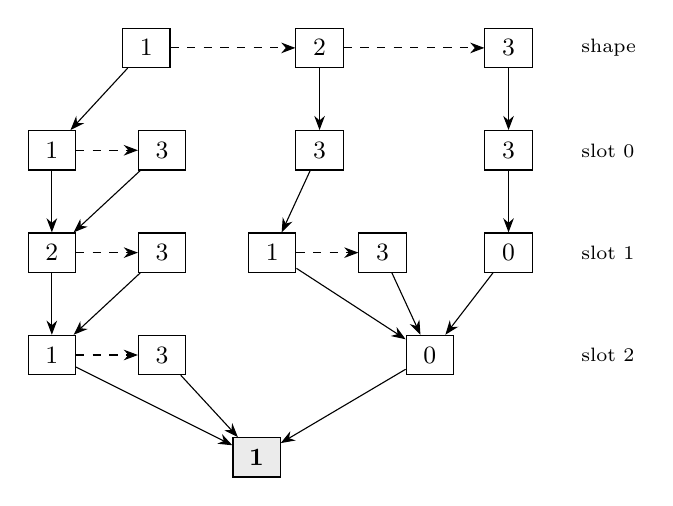
\begin{tikzpicture}[
  n/.style={draw,rectangle,minimum width=6mm,minimum height=5mm,inner sep=1pt,font=\small},
  dn/.style={-{Stealth[length=1.8mm]}},
  rt/.style={-{Stealth[length=1.8mm]},dashed}]
  % level 0: shape
  \node[n] (a1) at (0,0) {1};
  \node[n] (a2) at (2.2,0) {2};
  \node[n] (a3) at (4.6,0) {3};
  % level 1: slot 0
  \node[n] (b1) at (-1.2,-1.3) {1};
  \node[n] (b2) at (0.2,-1.3) {3};
  \node[n] (b3) at (2.2,-1.3) {3};
  \node[n] (b4) at (4.6,-1.3) {3};
  % level 2: slot 1
  \node[n] (c1) at (-1.2,-2.6) {2};
  \node[n] (c2) at (0.2,-2.6) {3};
  \node[n] (c3) at (1.6,-2.6) {1};
  \node[n] (c4) at (3.0,-2.6) {3};
  \node[n] (c5) at (4.6,-2.6) {0};
  % level 3: slot 2
  \node[n] (d1) at (-1.2,-3.9) {1};
  \node[n] (d2) at (0.2,-3.9) {3};
  \node[n] (d3) at (3.6,-3.9) {0};
  \node[n,fill=black!8] (T) at (1.4,-5.2) {$\mathbf 1$};
  \draw[rt] (a1) -- (a2); \draw[rt] (a2) -- (a3);
  \draw[rt] (b1) -- (b2);
  \draw[rt] (c1) -- (c2); \draw[rt] (c3) -- (c4);
  \draw[rt] (d1) -- (d2);
  \draw[dn] (a1) -- (b1); \draw[dn] (a2) -- (b3); \draw[dn] (a3) -- (b4);
  \draw[dn] (b1) -- (c1); \draw[dn] (b2) -- (c1);
  \draw[dn] (b3) -- (c3); \draw[dn] (b4) -- (c5);
  \draw[dn] (c1) -- (d1); \draw[dn] (c2) -- (d1);
  \draw[dn] (c3) -- (d3); \draw[dn] (c4) -- (d3); \draw[dn] (c5) -- (d3);
  \draw[dn] (d1) -- (T); \draw[dn] (d2) -- (T); \draw[dn] (d3) -- (T);
  \node[font=\scriptsize,anchor=west] at (5.4,0) {shape};
  \node[font=\scriptsize,anchor=west] at (5.4,-1.3) {slot 0};
  \node[font=\scriptsize,anchor=west] at (5.4,-2.6) {slot 1};
  \node[font=\scriptsize,anchor=west] at (5.4,-3.9) {slot 2};
\end{tikzpicture}
\caption{The reachable states of \cref{ex:sym-par} as an LDD (derived by
hand; the five padding positions of the real vectors, each a single node
$0$, are left out). Solid: down; dashed: right. Values: $1 = \code{pre a
nil}$, $2 = \code{pre b nil}$, $3 = \code{nil}$, $0$ = no slot; shapes
$1 = \sigma_1$, $2 = \sigma_2$, $3 = \sigma_3$. The 15 nodes hold 11
vectors: the 8 of $\{1\}\times\{1,3\}\times\{2,3\}\times\{1,3\}$, then
$(2,3,1,0)$, $(2,3,3,0)$, $(3,3,0,0)$. The nodes $2{\to}3$ at level 2 and
$0$ at level 3 are shared.}
\label{fig:sym-ldd}
\end{figure}

\subsubsection{Relations}

A relation is an LDD read through a \emph{meta} vector, one code per state
position, ended by $-1$ (\code{0xFFFFFFFF};
\locr{lib/ldd/ldd.ml}{73}{84}). For a set $S$ of vectors of length $n$,
a relation LDD $R$ and meta $m$, Sylvan's \code{lddmc_relprod} and
\code{lddmc_relprev} interpret each position $i$ by its code:

\begin{center}
\small
\begin{tabular}{@{}c l l l@{}}
\toprule
code & \code{Ldd.level} & levels of $R$ & meaning for $(w, w')$ \\
\midrule
0 & \code{Copy} & none & $w'_i = w_i$ \\
1, 2 & \code{Read}, \code{Write} & two: old, new & $R$ holds $w_i$, then $w'_i$ \\
3 & \code{Only_read} & one & $R$ holds $w_i$, and $w'_i = w_i$ \\
4 & \code{Only_write} & one & $R$ holds $w'_i$, $w_i$ arbitrary \\
5 & \code{Label} & one, no state position & skipped \\
$-1$ & (end) & & the remaining positions copied \\
\bottomrule
\end{tabular}
\end{center}

Writing $w \to_{R,m} w'$ when some sequence of $R$ matches $(w,w')$
under $m$:
\[
\mathrm{relprod}(S,R,m) = \{w' \mid \exists w\in S.\ w\to_{R,m}w'\},
\]
\[
\mathrm{relprev}(S,R,m,U) = \{w \in U \mid \exists w'\in S.\ w\to_{R,m}w'\}.
\]
The point of the meta is locality: a relation over $k$ touched positions
of an $n$-vector stores only those $k$ (or $2k$) levels, and one learned
tuple applies to every state that agrees on the read positions.
\code{Label} is bound and tested (\loc{test/ldd_tests.ml}{47}) but the
engine never uses it: it keeps one relation per label instead.

\subsubsection{The bound operations}

Every OCaml function and the C stub behind it
(\file{lib/ldd/ldd.mli}; \file{lib/ldd/ldd.ml} lines 5--24 for the
externals; \file{lib/ldd/ldd_stubs.c}):

\begin{center}
\small
\begin{tabularx}{\linewidth}{@{}>{\raggedright\arraybackslash}p{3.2cm} >{\raggedright\arraybackslash}p{3.6cm} >{\raggedright\arraybackslash}X@{}}
\toprule
OCaml (\file{ldd.mli}) & C stub (\file{ldd_stubs.c}) & Sylvan call, notes \\
\midrule
\code{init} (22) & \code{ml_ldd_init} (74--84) & \code{lace_start(workers, 1000000)};
  \code{sylvan_set_limits(mb MB, 1, 5)}; \code{sylvan_init_package};
  \code{sylvan_init_ldd}. Only the first call acts (static \code{started}).
  Defaults: 1 worker, 1024\,MB (\loc{lib/ldd/ldd.ml}{26}). \\
\code{empty}, \code{epsilon} (25, 28) & \code{ml_ldd_false}, \code{_true} (86--87) &
  $\mathbf 0$, $\mathbf 1$. \\
\code{cube} (32) & \code{ml_ldd_cube} (89--95) & \code{lddmc_cube} inside a Lace task
  (\code{cube_task}, 56); values checked in OCaml to lie in $[0,2^{32}-2]$
  (\locr{lib/ldd/ldd.ml}{29}{40}); width at most 4096 (\code{MAX_WIDTH}, 20). \\
\code{of_list} (36) & \code{ml_ldd_union_cubes} (97--104) & Blocks of 64 cubes by
  \code{lddmc_union_cube} in a task (58--70), merged by halves with
  intermediate sets released (\locr{lib/ldd/ldd.ml}{42}{58}). Row width is
  taken from the first row and not checked for the others. \\
\code{union}, \code{minus}, \code{inter} (38--40) & 106--122 &
  \code{lddmc_union}, \code{lddmc_minus}, \code{lddmc_intersect}. \\
\code{equal}, \code{is_empty} (41--42) & \code{ml_ldd_equal} (146) & Node identity
  (canonicity); \code{is_empty s} is \code{equal s (empty ())}. \\
\code{mem} (43) & \code{ml_ldd_mem} (148--153) & \code{lddmc_member_cube}. \\
\code{count} (46) & \code{ml_ldd_count} (142) & \code{lddmc_satcount} (a long double)
  as a float. \\
\code{nodes} (49) & \code{ml_ldd_nodes} (144) & \code{lddmc_nodecount}. \\
\code{elements} (52) & \code{ml_ldd_elements} (188--207) & A read-only walk
  (\code{walk}, 168--186) collecting at most \code{limit} rows
  (default 1000, \loc{lib/ldd/ldd.ml}{61}), in lexicographic order; the
  engine always passes \code{~limit:max_int}. \\
\code{rel_meta} (65) & via \code{cube_c} & The meta cube, codes then $-1$. \\
\code{relprod}, \code{relprev} (68, 72) & 124--134 & \code{lddmc_relprod},
  \code{lddmc_relprev} (with \code{within} as Sylvan's universe). \\
\code{project} (76) & \code{ml_ldd_project} (136--140) & \code{lddmc_project} with
  codes 1 keep, 0 quantify, $-2$ ``quantify the rest''
  (\locr{lib/ldd/ldd.ml}{91}{100}). \\
\code{product} (80) & \code{ml_ldd_join} (209--213) & \code{lddmc_join} with
  projections $1^{w}\,{-2}$ for $a$ and $0^{w}\,{-1}$ for $b$: since $b$
  has none of $a$'s positions, the join is $\{u\cdot v\}$
  (\locr{lib/ldd/ldd.ml}{104}{115}). \\
\code{release} (83) & \code{ml_ldd_release} (155--162) & \code{lddmc_deref} now;
  the value then holds $\mathbf 0$. \\
\code{table_usage} (87) & 217--227 & \code{sylvan_table_usage}'s filled count, and
  \code{llmsset_get_max_size} (the maximum, not the current size). \\
\code{gc} (91) & \code{ml_ldd_gc} (230--235) & \code{sylvan_gc}. \\
\code{reclaim} (96) & OCaml only & If the table is over half full,
  \code{Gc.full_major ()} then \code{gc ()} (\locr{lib/ldd/ldd.ml}{117}{123}). \\
\bottomrule
\end{tabularx}
\end{center}

Sylvan's own operations (\code{lddmc_union} etc.) are macros that
\code{RUN} a Lace task (\file{vendor/sylvan/src/sylvan_ldd.h}, e.g.\
line 106), so the stubs may call them from the OCaml thread; only
\code{lddmc_cube} and \code{lddmc_union_cube} are wrapped by hand
(\locr{lib/ldd/ldd_stubs.c}{1}{8}).

\subsubsection{Memory: who keeps what alive, and when it is freed}

\begin{itemize}
\item \textbf{One reference per OCaml value.} \code{wrap}
  (\locr{lib/ldd/ldd_stubs.c}{40}{46}) allocates a custom block with
  \code{caml_alloc_custom_mem(.., 4096)}, telling OCaml's GC that each value
  holds about 4\,KB outside the heap (so the major GC runs sooner), and
  takes \code{lddmc_ref} on the node. The finaliser
  (\locr{lib/ldd/ldd_stubs.c}{22}{25}) drops the reference.
  \code{compare} and \code{hash} are by node index
  (\locr{lib/ldd/ldd_stubs.c}{27}{33}), so OCaml's \code{=} on \code{Ldd.t}
  is set equality.
\item \textbf{Nodes are freed only by Sylvan's GC}, which runs on demand
  when the unique table fills during an operation, or by \code{Ldd.gc}. It
  frees every node not reachable from a reference. A dead OCaml value not
  yet finalised still holds its reference, so its nodes stay. Hence
  \code{release} (free now) and \code{reclaim} (finalise, then collect).
\item \textbf{When the table is full even after a collection,} Sylvan
  prints ``MDD Unique table full'' and calls \code{exit(1)}
  (\file{vendor/sylvan/src/sylvan_ldd.c}, lines 373--374 and 400--401). Inside
  Rocq this ends the whole process (and the proof with it); it is not an
  exception, so no tactic can report it.
  The size is fixed at the first \code{init}: 1024\,MB in the plugin
  (\loc{lib/learn/learn.ml}{858} calls \code{Ldd.init ()}), 256\,MB in
  \file{test/ldd_tests.ml}. There is no Rocq option to change it.
\item \textbf{Sylvan is never shut down.} Once started inside a Rocq
  process, its tables (and one Lace worker thread) live until the process
  ends; nodes from one command are collected by later GCs once their OCaml
  values are finalised.
\end{itemize}

What the engine releases explicitly is listed with each algorithm below.
The rewrite of the game for memory (Phase~4) was prompted by three-process
coarse-grained against fine-grained CADP filling the 1024\,MB table in the game's sixth
iteration, while its relation was only 114k nodes: dead intermediate sets
filled the rest.

\subsubsection{Building and testing}

\file{lib/ldd/dune} copies the C files of \file{vendor/sylvan/src} and
\file{vendor/lace/src} and compiles them
\emph{into the binding's own library} (\code{-O2 -std=gnu11
-D_GNU_SOURCE -w}), not into a separate C library: Rocq loads the plugin's
libraries as \code{.cmxs} with Dynlink, and a C archive's objects reach a
\code{.cmxs} only when the same link refers to them.
\file{lib/ldd/README.md} gives the upstream versions, the two
hand-written configuration headers (\file{lib/ldd/config/sylvan_config.h},
\file{lace_config.h}) and how to update. \file{test/ldd_tests.ml} checks counts, the set
operations, canonicity, large values, image and preimage with a copy
level, a labelled relation, projection, product, release, and locality:
two independent counters mod 100, one relation each, reach 10,000 states
in at most 202 nodes (\locr{test/ldd_tests.ml}{64}{89}).

\subsection{Learning relations: \texttt{lib/learn}}\label{sec:sym-learn}

\subsubsection{States as vectors}

All tables are shared by the two systems of a check, so that labels
compare (\code{tables}, \locr{lib/learn/learn.ml}{40}{52}): values,
shapes and labels each get an integer from 1 in order of first meeting
(\code{intern}, \locr{lib/learn/learn.ml}{91}{99}); 0 means ``no slot''.
Terms are hashed by \code{deep_hash} (\locr{lib/learn/learn.ml}{8}{21}),
a structural hash of the whole term consistent with \code{Constr.equal}:
\code{Hashtbl.hash} looks at 10 nodes only, and CADP's large terms that
differ deep down collided (stage 2c).

A state $t$ of a system with \code{width} $w$ is the vector
\[
\mathrm{enc}(t) = [\,\#\mathit{shape};\ \#v_0;\ \dots;\ \#v_{k-1};\
0;\ \dots;\ 0\,] \in \N^{w+1}
\]
from \code{Skeleton.split} (\code{encode},
\locr{lib/learn/learn.ml}{117}{138}; \code{decode} rebuilds,
\locr{lib/learn/learn.ml}{140}{146}), each slot at its place in the
shape's order (below). If a state has more than $w$ slots,
\code{Too_wide n} is raised (also from \code{make_summand} and
\code{split_target}), and \code{check} restarts that system's exploration
with width $\max(n, 2w)$ (\code{run_explore},
\locr{lib/learn/learn.ml}{1632}{1635}). The initial width is 8.

\paragraph{The order of the slots.} A slot need not sit at its own
index: since 9 November 2026, for a system whose summands all keep the
start's shape, the slots go in order of how many summands read or write
them, most first, ties left to right (\code{explore},
\locr{lib/learn/learn.ml}{1141}{1187}). Each summand's positions are
then near the front and the rest of the vector is copied, which is what a
static variable ordering over the dependency matrix aims
for~\cite{meijer-vdpol16}; in CADP the shared memory comes first, each
process's own slots after. The order is a table per shape
(\code{perm}, \code{pos}; \code{pos_of} and \code{slot_at},
\locr{lib/learn/learn.ml}{69}{89}), read by \code{encode},
\code{decode}, the summands' codes and the partial terms, and handed to
the summands' codes and the partial terms. \code{MEBI_ORDER=off} keeps
each slot at its index.

\subsubsection{The interpreter}\label{sec:sym-interp}

A summand is learned on a \emph{partial term}: the source shape with the
read slots' values and, in every other slot $i$, a placeholder
\code{Meta i} (\code{partial}, \locr{lib/learn/learn.ml}{994}{1008}).
\code{fire c lts src chain} (\locr{lib/learn/learn.ml}{295}{325}) follows
the chain:

\begin{shell}[mathescape=true]
fire(lts, src, chain):                                   (learn.ml:259-312)
  []           -> []
  "<..>" :: r  -> if src has a placeholder: Stuck
                  else [(l, t, r) | (l, t) in steps(lts, src)]
  name :: r    -> $\rho$ := the rule called name;  b := cmatch($\rho$.src, src)   (No_match -> [])
                  for each b' in prems($\rho$.premises, b, r):
                      (compute(subst b' $\rho$.lbl), compute(subst b' $\rho$.tgt), rest)
prems(Decide w :: ps)        -> if compute(subst b w) = true then prems(ps) else []
prems(Opaque _ :: _)         -> Stuck
prems(Step L' s l t :: ps)   -> for each (l', t', r') in fire(L', compute(subst b s), chain):
                                   cmatch l against l', t against t'; prems(ps)
steps(lts, src):  memoised per (lts, src)
  if depth $\ge$ 64: Unfollowable(lts, src)
  else interp(lts, src), or Unfollowable(lts, src) on Stuck   (interpreted += 1)
interp(lts, src): every rule of lts, as fire, premises by prems_all  (learn.ml:345-385)
\end{shell}

\begin{itemize}
\item \code{cmatch} (\locr{lib/learn/learn.ml}{167}{202}) is first-order
  matching of a rule's source pattern against a term. A constructor
  pattern against a placeholder raises \code{Stuck}; a variable bound twice
  to a term with a placeholder raises \code{Stuck}; a closed non-constructor
  pattern (a constant such as \code{Acquire}) is compared with the term
  after \code{nf_all}.
\item \code{compute} (\locr{lib/learn/learn.ml}{212}{227}) normalises a
  closed term with \code{nf_all}; around placeholders it only descends
  through constructor applications, and raises \code{Stuck} on anything
  else or on \code{unbound} (\code{Meta 1000000}, a variable nothing
  bound, \loc{lib/learn/learn.ml}{199}). So a placeholder in the result
  means ``that slot carried unchanged''.
\item Two exceptions with distinct meanings: \code{No_match} (this rule
  does not apply) and \code{Stuck} (the interpreter cannot decide: on a
  closed term, the step is \code{Unfollowable}, an error). \code{max_depth} $= 64$ (\loc{lib/learn/learn.ml}{281}) stops a
  rule whose premise steps from its own source from recursing forever.
\item Rules of other LTSs are read lazily through \code{rules_of}
  (\locr{lib/learn/learn.ml}{283}{291}).
\end{itemize}



\subsubsection{Summands' relations and meta codes}

Each summand of a source shape becomes a record
(\locr{lib/learn/learn.ml}{410}{420}) with its chain, its projection
\code{keep} (position 0, the shape, always; then the read slots), its
static codes, the projections already learned (\code{seen}), its
relations, and the projections that escaped. The static codes come from
\code{make_summand} (\locr{lib/learn/learn.ml}{443}{500}). With $k_s$ the
source's slots, $k_t$ the target's, and \emph{same} whether the target
shape equals the source shape:
\[
\mathrm{reads} = \mathrm{reads}_{\mathrm{skeleton}} \cup \{ i \mid
  \text{target slot } j \text{ is } \mathsf{Moved}\ i,\ \neg(\mathit{same}
  \wedge i = j) \}
\]
(a value moved to another place counts as read: its new place holds the
old value), and position $p$ gets (LTSmin's read, write and copy
dependencies~\cite{meijer14})
\[
\mathrm{code}(0) = \begin{cases}\mathsf{RO} & \mathit{same}\\
\mathsf{RW} & \text{else}\end{cases}
\qquad
\mathrm{code}(1+j) = \begin{cases}
\mathsf{RW} & j\in\mathrm{reads},\ \mathrm{written}(j)\\
\mathsf{RO} & j\in\mathrm{reads},\ \neg\mathrm{written}(j)\\
\mathsf{WO} & j\notin\mathrm{reads},\ \mathrm{written}(j)\\
\mathsf{Copy} & \text{else}
\end{cases}
\]
where $\mathrm{written}(j)$ holds if $j<k_t$ and target slot $j$ is not
$\mathsf{Moved}\ j$ in the same shape, or $k_t \le j < k_s$ (the slot
disappears and is padded to 0). \code{levels}
(\locr{lib/learn/learn.ml}{469}{477}) maps $\mathsf{RW}$ to
\code{[Read; Write]}, $\mathsf{RO}$ to \code{Only_read}, $\mathsf{WO}$ to
\code{Only_write}, $\mathsf{Copy}$ to \code{Copy}.

\subsubsection{Learning a projection}

\code{learn sm frontier visited} (\locr{lib/learn/learn.ml}{625}{746}):

\begin{shell}[mathescape=true]
fresh := project(frontier, sm.keep) $\setminus$ sm.seen
for each pv in fresh with pv[0] = sm.sid:                   projections += 1
  results := fire(lts, partial(shape, sm.keep, pv), sm.chain)    (Stuck -> escape pv)
  for each (l, t): split t into (target shape, slots: Mv i | Val v)    (split_target, 523-535)
  if some Mv i with i $\ne$ j and slot i unread: escape pv     (a move of an unread slot)
  else for each result:
    widen the static codes where this result writes more        (needs, 695-716):
      RO $\to$ RW, Copy $\to$ WO   if position written;  WO $\to$ Copy  if not
    tuple := per code: RW (old,new), RO old, WO new, Copy nothing
    batch[(codes, label)] += tuple
sm.seen $\cup$= fresh;  add batch as one LDD per (codes, label)       (add_rel, 491-500)
escaped projections: learn their whole states among visited  (learn_global, 589-618)
\end{shell}

\begin{itemize}
\item A position ``needs'' a write (\locr{lib/learn/learn.ml}{695}{706})
  if it is the shape and the shape changed, a slot moved from elsewhere, a
  value that is not the read slot's own old value, or a slot beyond the
  new shape but within the old (padded to 0). A read slot comes back from
  the interpreter as a value, not a placeholder, so ``value equal to the
  old one'' is no write: this misclassification caused all 37,584 of
  Test4's escapes in stage 2b (\file{doc/learn.md}, stage 2c item 1).
\item Hence one summand may hold several relations, one per (codes,
  label): a result whose shape changed at run time (a dynamic summand,
  e.g.\ a \code{tfix} unfolding into a \code{tpar}) goes into a relation
  with more positions written.
\item \textbf{Escapes.} \code{learn_global} decodes each whole state and
  fires the chain on it; if that is \code{Stuck} too, it takes
  \emph{all} the state's steps from \code{steps} (a superset of the
  summand's, ``always correct to add''). Its tuples have every position
  $\mathsf{RW}$. Escapes cost time, never correctness: every tuple added is
  a real step. After stage 2c, escapes were 0 on every measured file.
\end{itemize}

\paragraph{A placeholder in a value is not checked.} \code{split_target}
interns any non-placeholder slot value as a value, even one that contains
a placeholder deeper inside (e.g.\ a non-structural constructor applied
to an unread slot). That would intern an open term as a state value.
Skeleton's \code{computed_reads} is meant to make every slot a computed
value depends on ``read'', so this should not arise; the code relies on
that analysis and does not check it (\locr{lib/learn/learn.ml}{526}{533}).

\begin{example}[\cref{ex:sym-par}, learned]
For \code{s_parl; s_parl; <step>} the codes are $[\mathsf{RO};
\mathsf{RW}; \mathsf{Copy};\dots]$ and the projections are $(1, v_0)$.
On $(1,1)$ the partial term is
\code{par (par (pre a nil) ?1) ?2}; \code{fire} matches \code{s_parl}
twice, then \code{steps step (pre a nil)} interprets \code{s_pre}: label
\code{Some a}, target \code{nil}. The result
\code{par (par nil ?1) ?2} splits to $[\mathsf{Val}\,3; \mathsf{Mv}\,1;
\mathsf{Mv}\,2]$, so the relation for label \code{Some a} is the single
tuple $(1;\,1,3)$: ``in shape 1, slot 0 goes from 1 to 3, the rest is
copied''. It applies to all four states $(1,1,\ast,\ast)$ at once.
For \code{s_parl; s_end} every position $0..3$ is $\mathsf{RW}$ (the shape
changes, slot 2 moves to slot 1, slot 2 is padded); its relation, label
\code{None}, is $\{(1,2,\,3,3,\,3,v,\,v,0) \mid v \in\{1,3\}\}$, learned on
the projections $(1,3,3,v)$; other projections do not match
\code{par nil nil} and give nothing.
\end{example}

\subsubsection{Chained exploration}

\code{explore} (\locr{lib/learn/learn.ml}{972}{1242}) is breadth-first with
LTSmin's~\cite{kant15} \emph{chaining}: within a round, each summand in turn is learned
on and applied to the round's frontier grown by what the summands before
it found.

\begin{shell}[mathescape=true]
visited := frontier := {enc(start)}
while frontier $\ne\emptyset$:                                      (763-809)
  reclaim()
  sms := summands of the shapes in frontier     (766-771)
  cur := frontier;  added := $\emptyset$
  for sm in sms:
    learn(sm, cur, visited)
    f := $\bigcup_{r\in sm.rels}$ relprod(cur, r.rel, meta(r.codes)) $\setminus$ visited
    visited, cur, added $\cup$= f;  learn escaped projections' states in f
  frontier := added
\end{shell}

Released explicitly: the projection, \code{fresh}, the old \code{seen},
\code{next}, \code{f}, and the previous \code{visited}, \code{cur},
\code{added}, \code{frontier}. Not released (left to finalisers): the meta
cubes built per application (\loc{lib/learn/learn.ml}{785}) and the
shape projection (\loc{lib/learn/learn.ml}{769}). Chaining pays where
summands feed each other (Proc's Test1: 3--6 rounds) and not on CADP's
fine-grained model (2 summands, 81 rounds).

\paragraph{A bug fixed on 2026-11-08: 1000 shapes.} The shapes of a
frontier were listed with \code{Ldd.elements} at its default \code{limit}
of 1000. A frontier with more than 1000 distinct shapes would silently have
skipped the summands of the others; their states would have stayed in
\code{visited} without successors, giving a smaller reachable set and
possibly a wrong verdict (no measured example has more than 9 shapes).
Found by the first draft of this report; now every call in the file passes
\code{~limit:max_int} (\loc{lib/learn/learn.ml}{769}; also 730, 745, 759,
1087, 1104, 1118). \code{Ldd.elements}'s default is still 1000, a trap for
a future caller.

\paragraph{Why it is complete.} Each state enters some \code{cur} exactly
once, when it is new; every projection of it is then learned (or escaped
and learned whole), and a projection's results, once learned, are all its
steps. So a later state with an already-seen projection gets its
successors from the existing tuples, and no earlier state can gain
successors later. Soundness rests on every tuple being a real step: from
the interpreter, which follows the rules.

\paragraph{Saturation, measured and set aside}~\cite{ciardo01} (Phase~3; \file{doc/future-work.md},
``Saturation for the symbolic route''). On three-process coarse-grained CADP
against \code{spec_lts}: 119\,s interpreting summands (1.92M projections),
16\,s other learning, \textbf{0.25\,s applying relations}, 0.2\,s the
game. Saturation speeds up the application of relations, which is under
1\% of the time on every example.

\subsection{The game, symbolically: weak and strong}\label{sec:sym-game}

Let $\to_A$ and $\to_B$ be the learned relations (the union over
summands, per label), $\Reach_A$, $\Reach_B$ the explored sets, and
\[
\Uni = \Reach_A \times \Reach_B
\]
built by \code{Ldd.product} (\loc{lib/learn/learn.ml}{887}); a pair is the
concatenation of $A$'s vector and $B$'s. A relation of $B$ acts on pairs
with $|A|$ copy codes in front (\code{rels_of ~offset},
\locr{lib/learn/learn.ml}{890}{909}); a relation of $A$ needs no padding,
since positions after the meta's end are copied.

\paragraph{The silent label, and \code{?strong}.} \code{tau}
(\locr{lib/learn/learn.ml}{1327}{1343}) is an \code{int option}:
\begin{ocaml}
  let tau =
    let none = Rocqlib.lib_ref "core.option.None" in
    if strong
    then None
    else
      CTbl.fold (fun t i acc -> match Constr.kind (fst (Constr.decompose_app t)) with
        | Constr.Construct (c, _) when (* c is None *) ... -> Some i
        | _ -> acc) tb.labels None
\end{ocaml}
In weak mode ($\mathit{strong}=\mathsf{false}$, the default) it is the
intern number of the label whose head constructor is \code{None}, found by
scanning the shared label table, or \code{None} if no reachable step is
silent. In strong mode it
is \code{None}: no label is silent, and a \code{None}-labelled step is an
ordinary label like any other. Write $\tau$ for the silent label when
there is one; everything below is defined for both modes.

\begin{definition}[The game]
For $Z\subseteq\Uni$ and a side $X\in\{A,B\}$ (the other side's component
fixed):
\begin{align*}
\pre^X_l(Z) &= \{ (p,q)\in\Uni \mid X\text{'s component steps by } l
  \text{ into a pair of } Z\} \\
T_X(Z) &= \begin{cases} \mu Y.\ (Z\cap\Uni) \cup \pre^X_\tau(Y) &
  \text{weak, with a silent label } \tau\\
  Z\cap\Uni & \text{strong (or no silent label)} \end{cases} \\
\Ok^X_l(Z) &= \begin{cases} T_X(Z) & l = \tau \\
  T_X(\pre^X_l(T_X(Z))) & l \ne \tau \end{cases}\\
\Bad_{A\to B}(Z) &= \textstyle\bigcup_{l\in L_A} \pre^A_l(\Uni \setminus \Ok^B_l(Z))
\end{align*}
($T_X(Z)$: $X$ reaches $Z$ by $\tau^\ast$; $\Ok^X_l(Z)$: $X$ answers $l$
weakly into $Z$; in strong mode there is no $l=\tau$ case), and
$\Bad_{B\to A}$ symmetrically. With $F_{\mathrm{sim}}(Z) = Z\setminus
\Bad_{A\to B}(Z)$ and $F_{\mathrm{bis}}(Z) = Z \setminus (\Bad_{A\to
B}(Z)\cup\Bad_{B\to A}(Z))$, the result is $Z^\ast = \nu F$, computed as
$Z_0 = \Uni$, $Z_{i+1} = F(Z_i)$ until $Z_{i+1} = Z_i$. The verdict is
$(\mathrm{enc}(s_A),\mathrm{enc}(s_B)) \in Z^\ast$.
\end{definition}

Unfolded: $(p,q)\in\Bad_{A\to B}(Z)$ iff $p\to^l_A p'$ for some $l, p'$
and there is no $q'$ with $q \wtr{l} q'$ (for $l=\tau$: $q\to_\tau^\ast
q'$) and $(p',q')\in Z$. This is exactly \code{simF}
(\locr{theories/Bisimilarity.v}{60}{64}): a strong move answered by a
\code{weak} move (\locr{theories/Bisimilarity.v}{44}{47}), the silent
case allowing zero steps; \code{bisimF}
(\locr{theories/Bisimilarity.v}{212}{218}) adds the converse.

\paragraph{The strong game.} With no silent label, $T_X(Z) = Z\cap\Uni$, so
$\Ok^X_l(Z) = \pre^X_l(Z)\cap\Uni$ for every $l$, and
\[
F^{s}_{\mathrm{sim}}(Z) = Z \setminus \textstyle\bigcup_{l\in L_A}
  \pre^A_l\bigl(\Uni\setminus\pre^B_l(Z)\bigr),
\qquad
F^{s}_{\mathrm{bis}}(Z) = F^{s}_{\mathrm{sim}}(Z) \setminus
  \textstyle\bigcup_{l\in L_B}\pre^B_l\bigl(\Uni\setminus\pre^A_l(Z)\bigr).
\]
Unfolded: $(p,q)$ is removed iff $p\to^l_A p'$ and no $q\to^l_B q'$ has
$(p',q')\in Z$ (and, for bisimilarity, symmetrically). The result is again
$Z^\ast = \nu F^{s}$, iterated from $\Uni$. Its post-fixpoints are exactly
the relations satisfying \code{ssimF} (\code{sbisimF}) of
\locr{theories/Bisimilarity.v}{361}{376}: a step, \code{None} included,
answered by one step with the same label. Since the same code computes both,
the strong game is the weak one with $\tau^\ast$ replaced by the identity;
nothing else changes (\code{bad} still takes the answerer's
\code{tau_star} once, which is now $Z\cap\Uni$, and the test
\code{Some l = tau} is never true).

\begin{proposition}
$F$ is monotone and $F(Z)\subseteq Z$, so the iteration from $\Uni$
reaches $\nu F$ in at most $|\Uni|$ steps. $\nu F$ is the largest weak
simulation (for $F_{\mathrm{bis}}$: the largest weak bisimulation)
contained in $\Uni$ of the learned LTSs. If the learned relations are
exactly the Rocq LTS's steps on reachable states, the verdict is
\code{weak_sim} (\code{weak_bisimilar}) of the start terms; for
$F^{s}$, \code{strong_sim} (\code{strong_bisimilar}).
\end{proposition}
\begin{proof}[Sketch]
$Z\subseteq Z'$ gives $T_X(Z)\subseteq T_X(Z')$, hence
$\Ok(Z)\subseteq\Ok(Z')$ and $\Bad(Z)\supseteq\Bad(Z')$. A post-fixpoint
$R\subseteq F(R)$ is a relation in $\Uni$ whose every move is answered
into $R$, i.e.\ a weak (bi)simulation; the greatest fixpoint contains all
of them. Every successor of a reachable state is reachable, so
restricting to $\Uni$ loses no pair a (bi)simulation from the start pair
needs.
\end{proof}
This argument is not mechanised. What is checked in Rocq is the
certificate (\cref{sec:prooflog}), not the engine.

\paragraph{With LDD operations} (\locr{lib/learn/learn.ml}{927}{1024}):
\begin{shell}[mathescape=true]
pre(X, l, S)       = $\bigcup$ over X's relations r with label l: relprev(S, r, meta, within = U)
tau_star(X, Z)     = Z := Z $\cap$ U;  if tau = None: Z            -- strong: the identity on U
                     fresh := Z
                     while fresh $\ne\emptyset$: p := pre(X,$\tau$,fresh); fresh := p $\setminus$ Z; Z $\cup$= fresh
bad(M, Ans, Z)     = tz := tau_star(Ans, Z)                 -- once per iteration, not per label
                     $\bigcup_{l\in L_M}$ pre(M, l, U $\setminus$ ok_l),   ok_$\tau$ = tz,  ok_l = tau_star(Ans, pre(Ans, l, tz))
                     -- strong: tz = Z $\cap$ U and ok_l = pre(Ans, l, tz) $\cap$ U for every l
gfp(Z)             = bd := bad(A, B, Z) [$\cup$ bad(B, A, Z) for Bisim]
                     Z' := Z $\setminus$ bd;  if Z' = Z then Z else gfp(Z')
verdict            = mem(gfp(U), start)
\end{shell}
A pair is one vector, the \emph{answering} side's positions first (for
\code{Sim}, $B$'s: $\Uni = \Reach_B \times \Reach_A$; for \code{Bisim},
where both answer, the narrower side's; \code{b_first},
\loc{lib/learn/learn.ml}{1305}), so that the answerer's relations, applied
most, need no copied prefix; \code{start} is the two start vectors in that
order. A relation applied at an offset copies the positions before it, and
its meta stops at its last touched position (\code{meta_levels},
\loc{lib/learn/learn.ml}{520}): past the end Sylvan carries the rest of
the vector unchanged.
\code{tau_star} (\locr{lib/learn/learn.ml}{1354}{1373}; the strong case is
\loc{lib/learn/learn.ml}{1356}) applies only the pairs new in each round.
\code{pre} is at \locr{lib/learn/learn.ml}{1344}{1350}, \code{labels_of} at
\loc{lib/learn/learn.ml}{1375}, \code{bad} at
\loc{lib/learn/learn.ml}{1385}, \code{gfp} at
\loc{lib/learn/learn.ml}{1414}, called from $\Uni$ at
\loc{lib/learn/learn.ml}{1444}; the verdict is \code{Ldd.mem} of the start
pair (\locr{lib/learn/learn.ml}{1555}{1560}). Each iteration starts with
\code{reclaim ()}. Intermediate sets are released as soon as they are
dead (\code{union_into}, \loc{lib/learn/learn.ml}{1337}); the meta
cubes in \code{rels_tbl} and \code{uni} are not. Each iteration recomputes
the whole of $\Bad(Z)$; nothing is incremental across iterations
(40--47 iterations on CADP).

\subsection{\texttt{Learn.check} and its report}\label{sec:sym-check}

\begin{ocaml}
val check : Environ.env -> Evd.evar_map -> ?width:int
  -> ?strong:bool -> kind -> system -> system -> report
val pr : ?strong:bool -> kind -> report -> Pp.t
\end{ocaml}
(\file{lib/learn/learn.mli}.)
\code{kind} is \code{Bisim} or \code{Sim} (the first simulated by the
second); \code{strong} (default \code{false}) selects the strong game
(\cref{sec:sym-game}); it changes nothing before the game, so exploration,
the report's counts and the reachable sets are the same in both modes.
The tactics pass \code{~strong:true} for \code{sim}/\code{bisim} and
\code{false} for \code{weak_sim}/\code{weak_bisim}. \code{check} starts
Sylvan, builds the shared tables and interpreter context, explores $A$
then $B$, builds $\Uni$, runs the game, and, with the log on
(\code{proof_log}), repeats the last check with Sylvan's proof log open
(\cref{sec:prooflog}). The \code{report}:

\begin{center}
\small
\begin{tabularx}{\linewidth}{@{}l >{\raggedright\arraybackslash}X@{}}
\toprule
field & meaning \\
\midrule
\code{verdict} & start pair $\in Z^\ast$ \\
\code{states} & $|\Reach_A|$, $|\Reach_B|$ (floats, from \code{count}) \\
\code{pairs}, \code{nodes} & $|Z^\ast|$ and its node count \\
\code{labels} & distinct labels, both systems \\
\code{interpreted} & closed terms interpreted (shared context; counts
  from an aborted \code{Too_wide} attempt are included) \\
\code{projections}, \code{escapes} & per system \\
\code{summands}, \code{width}, \code{rounds} & per system; \code{width} is
  the vector length $w+1$ \\
\code{iterations}, \code{seconds} & of the game; wall-clock of the whole
  check \\
\bottomrule
\end{tabularx}
\end{center}

Exceptions: \code{Unfollowable}; and, outside OCaml, Sylvan's
\code{exit(1)} on a full table.

\subsection{The \texttt{debug} output}\label{sec:sym-debug}

Under \code{debug} $t$ for any of the four tactics, \code{prove} runs the
same \code{Learn.check} and, before testing the
verdict, prints \code{debug }$t$\code{: } followed by \code{Learn.pr
~strong k r} (\locr{lib/learn/learn.ml}{1142}{1195}) as a notice
(\file{src/user_tactics.ml}). The tactic then proceeds exactly as
without \code{debug}. There is no ``not run'' case any more: an exception
from the engine is the tactic's error. The format:
\begin{shell}
debug weak_bisim: symbolic (learned per summand, Sylvan): weakly bisimilar.
  reachable states: <a> and <b>; pairs in the relation: <n> (<k> nodes); labels: <l>
  summands: <sa> and <sb>; projections learned: <pa> and <pb> (escaped: <ea> and <eb>); steps interpreted: <i>
  vector widths <wa> and <wb>; exploration rounds: <ra> and <rb>; game iterations: <g>; <t>s
\end{shell}
The word is ``strongly'' under \code{~strong:true}
(\loc{lib/learn/learn.ml}{1143}); the verdict reads ``NOT \ldots\
bisimilar'', ``\ldots\ simulated'' or ``NOT \ldots\ simulated'' otherwise
. The goal checks of \code{prove}
(closed terms, LTS-shaped inductives) run first, so the engine never sees
an open goal.

\subsection{Limits}\label{sec:sym-limits}

\begin{itemize}
\item A closed premise's steps are interpreted from its LTS's rules to a
  depth of 64; a step the interpreter cannot follow (a rule whose source
  is not a pattern it can match, or a premise stepping from its own source
  without end) is an error, \code{Learn.Unfollowable}.
\item An LTS must be an inductive \code{M -> option A -> M -> Prop} without
  parameters.
\end{itemize}

\endgroup

\section{Terms as containers, and decision diagrams}\label{sec:containers}

A state is a closed Rocq term; a decision diagram stores sets of integer
vectors of one length. This section says how one becomes the other, and
why the way it is done is the theory of \emph{containers}~\cite{abbott05}:
the code is organised along that theory (\file{lib/skeleton/container.ml},
\file{lib/learn/learn.ml}, ``Serialisation''), which lets one encoding
serve systems whose states have several shapes.

\subsection{Containers}

A container $S \lhd P$ is a set of \emph{shapes} $S$ and, for each shape
$s$, a set of \emph{positions} $P(s)$. Its extension is the functor
\[
  [\![ S \lhd P ]\!](X) \;=\; \Sigma\, s \in S.\; (P(s) \to X),
\]
an element of which is a shape and a value in $X$ at each of its
positions. Strictly positive types are the initial algebras of
containers, and containers are closed under the usual constructions, the
free monad among them~\cite{abbott05}; with positions that carry types,
they are indexed containers~\cite{altenkirch15}.

\subsection{Three stages}

\paragraph{The term language} (\code{Container.view}). A closed term is a
constructor applied to parameters and fields, or something else (a value
that is not a constructor application). This stage knows nothing of the
rules.

\paragraph{Refinement by the rules} (\code{Container.split},
\code{Skeleton.classify}). A constructor is \emph{structural} if some rule
keeps it in place: it occurs in the rule's source and the same
constructor is at the same position of its target
(\cref{sec:sym-skeleton}). Write the state type as $T = \mu X.\, F_s(X) +
F_v(X)$, with $F_s$ the structural constructors and $F_v$ the others. Then
\[
  T \;\cong\; F_s^{*}(V),
\]
where $F_s^{*}$ is the free monad on $F_s$ and $V$ the terms whose head
is not structural. The free monad on a container is a container: its
shapes are the finite trees of structural constructors with holes, its
positions the holes. A term is therefore a shape (its top part made of
structural constructors), and a value at each position (the subterm
where that part stops), and the split is canonical: no value starts with
a structural constructor. Positions are \emph{paths} from the root (field
indices), not slot numbers.

The rules also classify each summand (a rule chain from a shape,
\code{Skeleton.kind}), and the three classes are the three kinds of map
on container elements:
\begin{itemize}
\item \textbf{local} (the shape stays): the identity on shapes, a new
  value at some positions;
\item \textbf{structural} (the shape changes, values are moved or
  dropped: $0 \mid 0 \to 0$, Proc's \code{do_par_end} and \code{do_assoc}):
  a container morphism, a map on shapes and a renumbering of positions;
\item \textbf{dynamic} (a computed value has structure, as a process that
  becomes a parallel composition): the value is itself an element of
  $F_s^{*}(V)$, and the state is flattened by the free monad's
  multiplication $F_s^{*}F_s^{*} \Rightarrow F_s^{*}$; the new shape is
  known only with the value.
\end{itemize}

\paragraph{Serialisation} (\file{lib/learn/learn.ml}). A shape becomes a
number, a position (a path) a vector index, a value a number (tables
built as the engine meets them, \code{0} meaning ``no position here''). A
state is the vector $[\textit{shape}; \textit{value at each position}]$,
padded to the system's width (8 positions to start with, doubled when a
state needs more). A path is numbered the first time a shape of the
system has it, in the order of its slots' use for the start shape
(\cref{sec:sym-learn}), so \emph{the same path has the same index in every
shape}: a step that changes the shape at one place leaves every value
elsewhere at its index, and the engine's relation copies those indices
instead of reading them.

\subsection{Decision diagrams are sets of container elements}

A list decision diagram (\cref{sec:sym-ldd}) over such vectors is a set
of serialised container elements, and its structure follows the
container's:
\begin{itemize}
\item its first level is the shape, a finite set: the diagram branches
  first on which shape a state has;
\item each further level is a position, and a node there holds the values
  that position takes; positions a shape does not have hold $0$, shared by
  all the states of that shape, so they cost one node;
\item the sharing of the diagram is the sharing of values among
  positions: a product of choices, one per position (independent
  processes), costs a sum of nodes, not a product;
\item a summand's relation is a relation on the positions it reads and
  writes, the others copied: on the container, a local map touches the
  positions at or below one place; a structural map, the shape and the
  positions it moves; a dynamic one, the shape and the positions of the
  structure the value became.
\end{itemize}
Because positions are paths, this locality is the container's: a change
below a place is a change of the vector below that place's indices. With
positions numbered as slots (left to right in the current shape, as until
10 November 2026), removing one leaf of the tree renumbered every leaf
after it, so a structural step rewrote values it did not touch, and the
engine had to learn it on whole states.

\subsection{Up to structural congruence}\label{sec:containers:upto}

\paragraph{Reorderings, found in the rules} (\code{Skeleton.reorderings}).
A rule is a \emph{reordering} if it has no premise, its label is
\code{None}, its source is a structure over pattern variables each used
once, and its target uses the same variables each once, otherwise
arranged: a container morphism that only permutes positions. That covers
commutation (Proc's \code{do_comm}), associativity (\code{do_assocl},
\code{do_assocr}), a swap or a rotation inside a structure. Only
reorderings whose inverse is one too are kept, so that they are
reversible; \code{do_par_end} ($0 \mid 0 \to 0$) is not one. When none is
found, or not the right ones, the command \code{MeBi Congruence lts
rules} names them by hand.

\paragraph{Proofs up to congruence: to design.} The engine can put every
reachable state in a class: the states it reaches by the congruence's
silent steps, and that reach it back. A certificate over pairs of classes
must answer the moves of \emph{every member} of a class, not only those of
a representative. Checking the representatives alone is unsound: with $b
\xrightarrow{\tau} a \xrightarrow{x} 0$ and $a \xrightarrow{\tau} b$, the
class $\{a, b\}$ would be ``matched'' by an inert state. This is weak
bisimulation up to a relation contained in mutual silent reachability,
with the whole class's moves checked, which makes it sound where ``up to
$\approx$'' is not~\cite{pous-sangiorgi11}. It covers weak goals only:
the silent path to the representative is not a one-step answer. The
certificate comes from the engine and is loaded as a proof term; Rocq
recomputes nothing (\cref{sec:optimisations}).

\section{The certificate: Sylvan's computation, typechecked}\label{sec:prooflog}

This section is the guide to how a goal's certificate is made and
checked. It assumes nothing from the rest of the report: every term is
defined here, with a small example, and every step can be reproduced from
the commands at the end (\cref{sec:prooflog:try}). The plan it follows is
\file{doc/certificate.md}.

\subsection{Why a certificate}\label{sec:prooflog:why}

\paragraph{Two ways to prove a fact.} Take the fact $2 + 2 = 4$ about the
natural numbers of Rocq. One way is to write a function that decides it,
for instance \code{Nat.eqb (2 + 2) 4}, which evaluates to \code{true}, and
let Rocq evaluate it: the proof is \code{eq_refl}, and Rocq's kernel accepts
it only after it has run the function itself. That is a \emph{proof by
computation} (or by reflection~\cite{boutin97}): the evidence is a
computation that the kernel repeats. The other way is to give the steps:
apply the lemma that $2 + 2 = 2 + (1 + 1)$, then the one that \dots, each
step a lemma applied to arguments, and the kernel only checks that each
application has the right type. That is a \emph{proof by certificate}: the
evidence is written down, and checking it is reading it.

\paragraph{Why it matters here.} The plugin's goals are about systems with
up to millions of states (three-process CADP: 7.9 million). The plugin
\emph{decides} a goal with a symbolic engine (\cref{sec:symbolic}), a
program in OCaml and C that is fast but not trusted. The certificate is
that program's own computation: the decision diagram library, Sylvan,
records each result it computes, the \emph{proof log}, and the plugin
writes each record as a lemma applied to its nodes. Rocq recomputes
nothing (CLAUDE.md, ``Hard rules''); \file{scripts/check_no_computation.py},
first in CI, fails on any use of \code{vm_compute}, a VM cast or the like.

\subsection{What the engine computes, from scratch}\label{sec:prooflog:background}

\paragraph{States as vectors.} The engine turns every state of a system
into a vector of natural numbers of fixed length (\cref{sec:containers}).
A pair of states, one from each system, is the two vectors put end to
end.

\paragraph{List decision diagrams.} A set of such vectors is stored as a
\emph{list decision diagram} (LDD)~\cite{blom-vdpol08}: a node holds a
value $v$, a child \emph{down} (the rest of the vectors that have $v$ at
this position) and a child \emph{right} (the vectors that have a larger
value here). Two leaves end the diagram: \code{D0}, the empty set, and
\code{D1}, the set holding only the empty vector. In Rocq
(\loc{theories/DdTree.v}{22}):
\begin{verbatim}
Inductive dd := D0 | D1 | Nd (v : N) (d r : dd).
\end{verbatim}
and \code{In_t x w} (\loc{theories/DdTree.v}{24}) says that the vector
\code{w} is in the set \code{x}: in \code{Nd v d r}, either \code{w} starts
with \code{v} and its rest is in \code{d}, or \code{w} is in \code{r}.
\emph{Example:} the set of vectors of length 1 $\{(1), (3)\}$ is
\code{Nd 1 D1 (Nd 3 D1 D0)}: a node with value 1 whose rest is the empty
vector, and to its right a node with value 3. In a node, the values along
a right chain always increase. Sylvan~\cite{vandijk-vdpol15} is the C
library that stores these nodes, each once (two equal nodes are the same
node, named by its index in Sylvan's table).

\paragraph{Operations on diagrams.} Sylvan computes with sets through a
few recursive operations: \emph{union}, \emph{minus} (difference),
\emph{intersect}, and the \emph{image} and \emph{pre-image} through a
relation (\code{lddmc_relprod}: the states one step after a set;
\code{lddmc_relprev}: the states one step before it). Each works node by
node, on the first values of its two arguments. Union, for instance
(\loc{vendor/sylvan/src/sylvan_ldd.c}{690}): if $a$ is empty, the result is
$b$ (and the other way round); if $a = b$, it is $a$; otherwise compare the
first values $v_a$ and $v_b$:
\begin{itemize}
\item $v_a < v_b$: the result is a node $v_a$, with $a$'s down, and to its
  right the union of $a$'s right with $b$;
\item $v_a > v_b$: the same with the roles swapped;
\item $v_a = v_b$: a node $v_a$ whose down is the union of the two downs
  and whose right is the union of the two rights (if the downs' union is
  empty, just the rights' union).
\end{itemize}
Sylvan remembers each result it computes in a \emph{cache}, keyed by the
operation and its arguments, so that a sub-computation met twice is done
once. (Before using the cache, its union swaps the arguments so that the
first has the larger index.)

\paragraph{The game.} To decide whether one system simulates another, the
engine solves a \emph{game} on pairs of states as a \emph{greatest
fixpoint} (\code{gfp}, \file{lib/learn/learn.ml}): start with $z$ = every
pair the engine explored (called \code{uni}); compute $\mathit{bad}(z)$,
the pairs of $z$ where the first system has a move the second cannot
answer (by silent steps, the same label, silent steps) into a pair of $z$;
remove them, $z := z \setminus \mathit{bad}(z)$; repeat until $z$ no longer
changes. The last iteration is the one where $z \setminus \mathit{bad}(z) =
z$: no pair of $z$ is bad, which is exactly what a simulation is. So
\emph{the last iteration is the proof}, if it can be written down. The
game takes 1 to 3 iterations on most goals, and up to 23 on
three-process CADP, of 6 to 97\,ms each.

The certificate does not log the game's iterations as they run: the
game's check is \emph{backward} (through the pairs from which an answer
exists, within the explored pairs \code{uni}), and a proof of it would
need \code{uni}, each system's exploration closed, and more. It logs the
same fact read \emph{forward}, as \emph{images}, which is the definition
of a simulation on $z$. For each relation $r$ of the \emph{mover} (the
system whose moves must be answered), with label $l$: every pair one
move after a pair of $z$ (the \emph{image} of $z$ by $r$) is a pair the
\emph{answerer} can answer. Those pairs, $\mathit{ok}_l$, come from $z$ by
the answerer's relations taken backwards (their \emph{inverses}: each
tuple's old and new values swapped): the pairs from which, after silent
steps, the label $l$ and silent steps, the answerer reaches $z$. The
inclusion is a difference that comes out empty. \emph{Example:}
$z = \{(p, s)\}$, the mover steps $p \xrightarrow{a} p'$ and the answerer
$s \xrightarrow{a} s'$, and $(p', s') \in z$. The image of $z$ by the
mover's $a$-relation is $\{(p', s)\}$; the image of $z$ by the answerer's
$a$-relation backwards is $\{(p', s)\}$ ($s$ steps to $s'$); and
$\{(p', s)\} \setminus \{(p', s)\}$ is empty. This check needs no
universe, no closure of the exploration, no intersection and no preimage
within a set. For a bisimilarity, each side in turn is the mover.

\subsection{The proof log}\label{sec:prooflog:log}

\paragraph{What is recorded.} While the log is open, each of the five
operations above writes one \emph{record} for each result it computes, at
the point where it offers the result to its cache
(\loc{vendor/sylvan/src/sylvan_ldd.c}{752} for union; 801, 925, 1167, 1738
for the others): which operation, which case it took (for union: whether
$v_a$ was below, equal to or above $v_b$; for the images, the kind of
position), its arguments and its result, all as node indices; 48 bytes.
Each worker thread of Sylvan writes its own buffer, so recording takes no
lock. By default the log stays in memory: each worker keeps its full
buffers in a list of its own, and the plugin reads the nodes the records
name from Sylvan's table itself. When the log is kept in a file instead,
closing it (\code{lddmc_log_close}) also writes every node reachable from
a recorded index (its value, down and right; 32 bytes), so the file can
be read without Sylvan. This is in the plugin's fork of Sylvan, on the
local branch \code{proof-log} of \file{vendor/sylvan} (three commits, on
10 and 11 November 2026; not pushed).

\paragraph{When.} The last iteration cannot be known in advance, so it is
repeated: once the fixpoint has finished, the engine clears Sylvan's cache
(else the repeated run would find every result there and record nothing),
turns Sylvan's garbage collection off (a collection would free nodes and
reuse their indices, which name the nodes in the log), grows Sylvan's
tables to their maximum first (Sylvan grows them only when it collects),
and runs, with the log open, the check as images
(\loc{lib/learn/learn.ml}{1459}). Logging every
iteration instead was rejected: the cache survives between iterations, so
every fact of every iteration would have to be kept, and CADP's 17 to 23
iterations would write many times what the proof needs.

\paragraph{Where, and whether.} Two options of the plugin
(\loc{src/user_tactics.ml}{186}) decide it:
\begin{itemize}
\item \code{Set MeBi Log Mode "off".} (the default) or \code{"keep"}:
  the log stays in memory while the tactic proves the lemma and is freed
  once the proof is built (\cref{sec:qed}), or it is written to a file and
  kept, for \code{MeBi Check Log}.
\item \code{Set MeBi Log Directory "<dir>".}: where the directory of
  the plugin's files goes; by default, next to the file being checked.
\end{itemize}
In memory, each of Sylvan's workers keeps its full buffers of records
in a list; after the log is closed, the plugin takes the records a
buffer at a time (\code{lddmc_log_take}), each buffer freed once taken,
and reads the nodes from Sylvan's own table, which collection leaves
alone until the facts are written. Nothing is written to disk. For a
file \code{F.v}, the plugin's files go in the directory \file{.F.v.mebi}
next to it (under dune, next to the copy dune checks, in
\file{_build/default}). A kept log of a lemma \code{L} is the one file
\file{.F.v.mebi/L.log}: the word \code{MEBILOG1}, the number of records,
the records, the number of nodes, the nodes. (A tactic is not told the
name of the lemma it proves; the plugin takes it from Rocq's internal
proof state, \loc{src/user_tactics.ml}{224}, and writes \code{goal} when
there is none.) \file{lib/ldd/proof_log.ml} reads such a file back.

\paragraph{Measured} (10 November 2026):

\begin{center}
\small
\begin{tabular}{@{}lrrrr@{}}
\toprule
 & records & nodes & logged check & memory \\
\midrule
two-process CADP & 10,533 & 6,234 & 0.17\,s & 0.51\,GB \\
three-process CADP & 488,067 & 233,068 & 0.82\,s & 1.33\,GB \\
\bottomrule
\end{tabular}
\end{center}

For three processes the file is 31\,MB, and the memory is the same as
without the log (the logged check's time includes growing Sylvan's
tables). Records by operation: image 270K, union 164K, minus 54K; no copy
nodes (a Sylvan feature the plugin does not use), and only the position
kinds copy, read, write and only-read. Those are the cases that need
lemmas.

\subsection{From records to facts}\label{sec:prooflog:facts}

\paragraph{What a fact is.} A \emph{fact} is one lemma applied to its
arguments, whose type the kernel checks. The lemmas about union and minus
are in \file{theories/DdTree.v}:
\begin{itemize}
\item \code{U a b c} (\loc{theories/DdTree.v}{131}): \code{c} holds exactly
  the vectors of \code{a} and those of \code{b};
\item \code{Mi a b R} (\loc{theories/DdTree.v}{183}): \code{R} is within
  \code{a}, and every vector of \code{a} is in \code{b} or in \code{R};
\end{itemize}
and there is one lemma for each case of Sylvan's operations:
\code{u_a0}, \code{u_b0}, \code{u_same} for the cases with an empty or an
equal argument, \code{u_lt}, \code{u_gt}, \code{u_eq}, \code{u_eq0} for the
three comparisons (the last when the downs' union is empty), and
\code{u_lt0}, \code{u_gt0}, \code{u_eq_d}, \code{u_eq_r} for a last step
folded into one fact (\cref{sec:prooflog:fit}); likewise \code{mi_*} for
minus. None of these lemmas needs to know that
$v_a < v_b$: they are about sets, not about order. So the facts of union
and minus need no comparison of numbers at all.

\paragraph{A worked example.} Take $a = \{(1), (3)\}$ =
\code{Nd 1 D1 (Nd 3 D1 D0)} and $b = \{(2)\}$ = \code{Nd 2 D1 D0}. Sylvan's
union compares 1 with 2: $1 < 2$, so the result is \code{Nd 1 D1 R} where
\code{R} is the union of \code{Nd 3 D1 D0} with $b$. That union compares 3
with 2: $3 > 2$, so it is \code{Nd 2 D1 R'} with \code{R'} the union of
\code{Nd 3 D1 D0} with \code{D0}, which is \code{Nd 3 D1 D0} (an empty
argument). The log holds two records (the two compared cases) and the
nodes; the facts, innermost first, are
\begin{verbatim}
f0 := u_b0 (Nd 3 D1 D0)
      : U (Nd 3 D1 D0) D0 (Nd 3 D1 D0)
f1 := u_gt (Nd 3 D1 D0) 2 D1 D0 (Nd 3 D1 D0) f0
      : U (Nd 3 D1 D0) (Nd 2 D1 D0) (Nd 2 D1 (Nd 3 D1 D0))
f2 := u_lt 1 D1 (Nd 3 D1 D0) (Nd 2 D1 D0) (Nd 2 D1 (Nd 3 D1 D0)) f1
      : U a b (Nd 1 D1 (Nd 2 D1 (Nd 3 D1 D0)))
\end{verbatim}
and the last says that the result, $\{(1), (2), (3)\}$, is the union.
(Sylvan stores a union under its own order of the two arguments; the
facts follow the order the caller asked for, each case having its mirror
image, so no fact is needed to turn one around.)

\paragraph{The translation} (\code{Dd_cert.write_log},
\loc{lib/certify/dd_cert.ml}{281}). For each union or minus record, the
translator finds the calls it made from the nodes' contents (which case
applies), and their facts from their own records; it checks that each
record's result is what its case says it must be (an error otherwise:
nothing is trusted), and writes the fact. It computes no set: every
result comes from the log.

\paragraph{Chunks.} A proof of three-process CADP has about 670,000
facts. Built as one term, the whole proof would sit in memory at once
before the kernel checks it. Instead, \code{MeBi Check Log} writes
the facts to a temporary file in pieces called \emph{chunks}, and reads
them back one chunk at a time (\file{lib/certify/dd_read.ml}); a proof's
facts, one chunk, go from the writer to the reader a line at a time,
with no file; each chunk is declared as its own
constant, which the kernel checks when it is declared. Here a chunk holds
up to 20,000 facts and the diagram nodes they mention, as local
definitions of its own proof; its statement is \code{True}, proved by
putting all its facts in a chain (\code{chk_u}, \code{chk_mi},
\code{chk_nil}, \loc{theories/DdTree.v}{264}), so that the kernel checks
every one. (A first design made each node a global constant: for three
processes, about 550,000 node constants took 1.8\,GB before the first chunk
was read, and the memory cap stopped it.)

\paragraph{The command and its numbers.} \code{MeBi Check Log "<file>".}
(\loc{src/user_tactics.ml}{289}) runs the translation and the reading on a
kept log, for testing; it proves no goal. Measured (10 November 2026):

\begin{center}
\small
\begin{tabular}{@{}lrrrrrr@{}}
\toprule
 & chunks & facts & nodes & written & read, checked & memory \\
\midrule
two-process CADP & 1 & 15,200 & 6,183 & 0.01\,s & 0.4\,s & 0.34\,GB \\
three-process CADP & 8 & 668,460 & 581,960 & 1.8\,s & 26.5\,s & 0.83\,GB \\
\bottomrule
\end{tabular}
\end{center}

For three processes, nodes are made again in each chunk that needs them
(233K distinct); the memory grows with each chunk, because Rocq keeps each
declared chunk until it writes the \file{.vo} file. One chunk instead of
eight (\code{MEBI_CHUNK_FACTS}) makes each node once and takes the same
time, but needs 1.42\,GB.

\subsection{Images, complete and sound}\label{sec:prooflog:images}

\paragraph{What they are.} A system's steps are stored as a
\emph{relation}: a diagram of \emph{tuples}, each saying how a step
changes a vector. For each position of the vector, a \emph{code} says what
the relation does there: \emph{copy} (the value stays, and the tuple holds
nothing for it), \emph{only-read} (the value stays and must equal the
tuple's), or \emph{read-write} (the tuple holds the old value, then the new
one). \emph{Example:} with codes (read-write, copy) and the tuple
$(1, 2)$, the vector $(1, 7)$ steps to $(2, 7)$: position 1 must hold 1 and
becomes 2, position 2 is copied. The \emph{image} of a set $x$ through a
relation is every vector one step after a vector of $x$: the image of
$\{(1,7), (3,7)\}$ is $\{(2,7)\}$ ($(3,7)$ has no step: no tuple reads
3). The \emph{inverse} relation swaps each tuple's old and new values:
$(2, 1)$; the image of $\{(2,7)\}$ through it is $\{(1,7)\}$, the vectors
one step \emph{before}. In Rocq the codes are \code{Copy}, \code{RO},
\code{RW} (\file{theories/DdTree.v}, \code{rstep},
\loc{theories/DdTree.v}{65}); Sylvan writes them as numbers per level of
the relation (0, 3, and 1 then 2), and the translator turns one into the
other.

\paragraph{Complete and sound.} A fact about a computed set can say two
things. \emph{Complete}: everything that belongs there is in the result
(the image of every vector of $x$ is in it: \code{PostC},
\loc{theories/DdTree.v}{281}). \emph{Sound}: everything in the result
belongs there (every vector of it is the image of a vector of $x$:
\code{PostS}, \loc{theories/DdTree.v}{526}). The proof needs the mover's
images complete (every move from $z$ is caught) and the answerer's sound
(whatever is in $\mathit{ok}_l$ really can be answered); \code{WlC} and
\code{WlS} are the same for the written part of a read-write position.

\paragraph{Why completeness needs comparisons.} Like union, Sylvan's image
walks the set's and the relation's right chains in parallel and skips a
node whose value cannot match. \emph{Example:} at a read-write position,
the set's first value is 1 and the relation's is 4. Every tuple reads a
value of at least 4 (values increase along a right chain), so no vector
starting with 1 has a step: Sylvan skips the set's node 1. For a sound
fact, skipping only drops candidates, so nothing needs to be shown
(\code{posts_x}, \code{posts_r}). For a complete fact, it must be shown
that what was dropped could not have had a step: that needs $1 < 4$, and
that the chains are sorted (the facts assume the sets sorted, \code{Srt}).
Each skip lemma of the complete direction takes the comparison Sylvan
made as a premise (\code{post_rw_lt}: $v_x < v_r$).

\paragraph{Comparisons as evidence.} A comparison such as $5 < 12$ is not
left for the kernel to compute: it is proved from the two numbers' binary
digits, one lemma per digit (\code{plt_*}, \code{nlt_pos}). In Rocq a
positive number is a list of binary digits read from the last:
$5 = $ \code{xI (xO xH)} (101), $12 = $ \code{xO (xO (xI xH))} (1100).
The proof of $5 < 12$ compares the last digits first: \code{plt_xI_xO}
says $2p+1 < 2q$ when $p < q$, so it needs $2 < 6$; \code{plt_xO_xO} says
$2p < 2q$ when $p < q$, so it needs $1 < 3$; and \code{plt_1_xI} says
$1 < 2q+1$. Three lemma applications; a number of $n$ binary digits needs
at most $n$.

\paragraph{When the relation ends early.} A relation of one system
leaves the other system's positions alone, and a relation touches only
some of its own. Its codes stop at its last touched position, and
\code{rstep} carries the positions after the last code unchanged, as
Sylvan does past the end of its meta. So an image at that point is the set
itself, in one fact (\code{post_end}, \code{posts_end},
\loc{theories/DdTree.v}{298}), with no step per node below it.

\paragraph{Related work.} Producing proof steps from a decision-diagram
package as it computes is the idea of Sinz and Biere~\cite{sinz-biere06},
and of Bryant and Heule~\cite{bryant-heule21}, where each BDD operation
emits clauses of an extended-resolution proof. Here each LDD operation's
case becomes the application of a lemma about sets, checked by Rocq's
kernel.

\subsection{Making three-process CADP fit}\label{sec:prooflog:fit}

Three-process CADP (7.9 million states) is the largest example. Each
change below was measured with \file{test/cert_tool.exe --log}, which runs
the translator alone and counts the facts of each lemma.

\paragraph{1. The check as images.} The game's own check, logged, needed
the explored pairs as a universe, each system's exploration closed,
intersections with the universe and complete preimages: 1.38M records,
2.46M facts. The forward check (\cref{sec:prooflog:background}) needs
none of these: 488K records.

\paragraph{2. The answering side first.} A pair is one vector. A relation
of the side whose positions come second must copy the other side's
positions before it reaches its own, one fact per node (\emph{copy
levels}). The answerer's relations are applied most (each label, each
silent round), so its positions come first (\loc{lib/learn/learn.ml}{1305};
for a bisimilarity, where both answer, the narrower side's), and each
meta stops at its relation's last touched position (\code{meta_levels},
\loc{lib/learn/learn.ml}{520}). The answerer's images are about 100 facts
in all.

\paragraph{3. Each image one way only: its role.} The logged run records
each image it makes at its top level with the way the proof uses it, 1
sound or 2 complete (\code{Ldd.log_top_relprod} in \file{lib/ldd}, the
fork's \code{lddmc_log_top}, operation 6 in the log), with the arguments
as passed, before Sylvan skips any node. The translator proves each image
only in that direction; a sound image needs no comparison.

\paragraph{4. Smaller tables in the translator.} The translator looks up a
record by its call (the operation and its arguments) in a table of its own
(\code{Itab} in \file{lib/certify/dd_cert.ml}: open addressing, the call
packed into two integers, the result and a ``called by another record''
bit in a third), about 32 bytes a record, and reads the log as a stream
(\code{Proof_log.read_iter}).

\paragraph{5. Comparisons shared within a chunk.} A complete skip needs the
comparison \code{a < b} of two node values, proved digit by digit
(\cref{sec:prooflog:images}). The same pair of values recurs: its proof is
made once per chunk (three processes: about 17,000 comparison facts).

\paragraph{6. A chain's last step folded in.} Many facts end a chain with
a fact about an empty set: the last written value of a read-write
position, then the empty rest (\code{wl_nd}, then \code{wl_r0}); a node
with no right sibling (\code{post_copy}, then \code{post_x0}); a union
with an empty or an equal side. A lemma for each such pair, proved once
from the two (\code{wl_last}, \code{post_copy_last}, \code{post_rw_last},
\code{u_lt0}, \code{u_gt0}, \code{u_eq_d}, \code{u_eq_r}, \code{mi_eq0d},
\code{mi_eq0r}), makes it one fact; and each union is proved in the order
of its arguments the caller asked for, with no fact to swap them. Three
processes: 963,941 facts down to 668,460, and 10\% less time (the folded
facts were the small ones).

\paragraph{7. The largest chunk first.} Rocq's kernel, when it checks a
constant, first copies its whole term into a hash-consed form (each
distinct subterm once, with a table), and keeps the types of the shared
parts. Measured on a chunk of 292,000 facts: its term took 52\,MB, and
checking it 510\,MB more, most of it live data, not garbage (a GC four
times as eager still needed 386\,MB). So a chunk's check needs memory in
proportion to its size, on top of what the chunks declared before it keep
(about 400 bytes a fact). One root alone can give 300,000 facts (one
image of the game's check), so chunks cannot simply be made smaller. Since the
check chunks need nothing from each other, \code{Dd_read} reads them
largest first: the largest check then meets the least memory held.
(Cutting a large root across chunks would need the nodes shared between
chunks as constants of their own; measured, a constant costs about 3\,KB,
too much for 233,068 nodes.)

\paragraph{Where the time goes.} Measured on three processes: the kernel
spends about 14\,\textmu s per node \code{let} and 28\,\textmu s per fact,
typing and hash-consing about equally. Binding the lists of codes and the
numbers as \code{let}s, or one chunk instead of eight, does not change the
total: what reduces it is fewer facts and fewer nodes.

\paragraph{Measured} (10 November 2026, \file{bench/prooflog.py}):
\begin{center}
\small
\begin{tabular}{@{}lrrrr@{}}
\toprule
 & decided & facts & checked in & memory at most \\
\midrule
two-process CADP & 0.8\,s & 15,200 & 0.7\,s & 0.34\,GB \\
three-process CADP & 22.9\,s & 668,460 & 29.5\,s & 0.83\,GB \\
\bottomrule
\end{tabular}
\end{center}
Before these changes, three processes took 2,461,163 facts, checked in
121\,s, 1.69\,GB at most. These are the facts alone (\code{MeBi Check
Log}); \cref{sec:qed} builds the proof of the goal from them.

\subsection{Trying it}\label{sec:prooflog:try}

For the two CADP examples, \file{bench/prooflog.py} does all of this
(after \code{dune build}): it copies each file into \file{_certify/log/},
turns the log on, stops once the engine has decided, checks each log in a
file of its own next to it, and prints the facts, times and memory. A
complete example is \file{test/rocq/LogTest.v} (in the build). In short:
\begin{verbatim}
Require Import MEBI.loader.
(* ... an LTS [step], then: *)
Set MeBi Log Mode "keep".
Example logged : weak_bisimilar step step (par A B) (par B A).
Proof. weak_bisim. Qed.
Set MeBi Log Mode "off".
MeBi Check Log ".LogTest.v.mebi/logged.log".
Print Assumptions mebi_log1_c1.
\end{verbatim}
\begin{enumerate}
\item The tactic decides the goal and proves it from the certificate
  (\cref{sec:qed}); with \code{"keep"}, the engine also leaves
  \file{.LogTest.v.mebi/logged.log}, and prints on standard error a line
  \code{[proof log] 628 records; the check as images: passes \dots}: the
  number of records, and that the check holds in the repeated run (it
  must pass).
\item \code{MeBi Check Log} prints the number of chunks, facts and nodes,
  the times, and the name of the last chunk's constant
  (\code{mebi_log1_c1}: the first use of the command in the file, its
  first chunk).
\item \code{Print Assumptions} on that constant must say ``Closed under the
  global context'': the facts use no axiom.
\end{enumerate}
To measure a large example, add \code{Set MeBi Log Mode "keep".} before its
proof and run it with \code{MEBI_CERT_STOP=decided} (stop once the engine
has decided) and \code{MEBI_CERT_STATS=1}; then check the log in a second
file. Run heavy examples under a memory cap (\file{CLAUDE.md}).

\subsection{What remains, and what was decided}\label{sec:prooflog:next}

\paragraph{Next} (\file{doc/certificate.md}; \cref{sec:status}): the
optimisations (\cref{sec:optimisations}); every example's proof already
ends with \code{Qed} (\cref{sec:qed:cost}).

\paragraph{Decided} (10 November 2026):
\begin{itemize}
\item \emph{one extra logged check}, not a log of every iteration;
\item \emph{the logged check as images}, the mover's complete and the
  answerer's sound by inverse relations, not the game's backward check:
  no universe, no closure of the exploration, no intersection, no
  complete preimage;
\item \emph{evidence, not re-checking}: where Sylvan has compared two
  values, the comparison is written as a proof built from the two
  numbers' binary digits, one lemma per digit, not as a computation the
  kernel repeats; lookups in lists are avoided by giving the element
  itself;
\item \emph{steps from the rules only}: the engine finds a term's steps by
  interpreting the LTS's rules; a step it cannot follow is an error;
\item \emph{side conditions with a \code{Decidable} instance}: proved
  through the instance, the kernel reducing its boolean once per step.
\end{itemize}

\section{The proof of a goal}\label{sec:qed}

\Cref{sec:prooflog} turned Sylvan's log into \emph{facts} about decision
diagrams. This section shows how the tactic turns those facts into a
proof of the goal itself, so that a file ends with \code{Qed}:
\begin{verbatim}
Example s1 : strong_sim step step (par A B) (par B A).
Proof. sim. Qed.
\end{verbatim}
The tactic decides the goal, Sylvan logs the decision (the
\emph{certificate}), and the tactic builds from it a proof that Rocq's
kernel checks at \code{Qed}. The proof uses no axiom: \code{Print
Assumptions s1} says ``Closed under the global context''
(\file{test/rocq/LogTest.v}). The section first defines what it needs
from Rocq (\cref{sec:qed:rocq}), then the example
(\cref{sec:qed:example}), the theorem the proof applies
(\cref{sec:qed:theorem}) and how each of its hypotheses is proved
(\cref{sec:qed:parts}); then how the pieces are put together
(\cref{sec:qed:assembly}), what Rocq computes (\cref{sec:qed:computes}),
how large goals were made to fit (\cref{sec:qed:fit}), the cost
(\cref{sec:qed:cost}) and how to try it (\cref{sec:qed:try}).

\subsection{What this section needs from earlier sections}\label{sec:qed:terms}

Each term below is defined, with an example, where the cross-reference
points; here is what each means for this section.
\begin{itemize}
\item A \emph{diagram} is a set of vectors of numbers, stored as a tree of
  \emph{nodes}: a node holds a value, a child \emph{down} (the rest of the
  vectors with that value) and a child \emph{right} (the vectors with a
  larger value there); the nodes reached by following right children
  from a node are its \emph{siblings} (\cref{sec:prooflog:background}).
\item A \emph{relation} is a diagram of \emph{tuples}: per position of a
  vector, a code says whether the step copies the value, reads it, or
  reads it and writes a new one, and the tuple holds the values read and
  written (\cref{sec:prooflog:images}).
\item The \emph{mover} is the system whose moves must be answered, the
  \emph{answerer} the one that answers them
  (\cref{sec:prooflog:background}).
\item A \emph{summand} is one way a state of a given shape can step: a
  chain of rules from the shape to a step of one of its slots
  (\cref{sec:containers}).
\item A \emph{fact} is one lemma of \file{theories/DdTree.v} applied to
  nodes and to other facts; it states what one of Sylvan's computations
  produced (a union, a difference, an image), and the kernel accepts it
  by typechecking (\cref{sec:prooflog:facts}). A \emph{chunk} is a batch
  of facts with the nodes they name, translated from the log together.
\end{itemize}

\subsection{What this section needs from Rocq}\label{sec:qed:rocq}

\paragraph{Terms, types, the kernel.} In Rocq a proof is a \emph{term}
whose \emph{type} is the statement it proves: a function taking a proof
of $A$ to a proof of $B$ proves $A \to B$. The \emph{kernel} is the small
part of Rocq that checks a term against its type (it \emph{typechecks}
it); nothing else is trusted. A \emph{tactic} is a program that builds
a term while a proof is in progress; \code{Qed} hands the finished term
to the kernel. The plugin's tactic builds the whole term at once and
gives it to Rocq without checking it (\code{exact_no_check}): the
kernel's check at \code{Qed} is the only one that counts.

\paragraph{Conversion.} While typechecking, the kernel may need two types
to be equal that are written differently, and it accepts them when one
\emph{computes} to the other: unfolding a definition, applying a function
to its argument, taking the matching branch of a \code{match}. This is
\emph{conversion}. \emph{Example:} if \code{val} looks a number up in a
table of values, a proof about \code{val 3} serves for the value stored
at 3, because \code{val 3} computes to it. Conversion is the only
computation the plugin's proofs rely on (\cref{sec:qed:computes}).

\paragraph{Definitions and \code{let}.} A \emph{constant} is a named
global definition: a body and its type. It is \emph{transparent} when
conversion may unfold it (a datum, such as a table of values, must be:
its contents matter), and \emph{opaque} when it may not (a proof: only its
statement matters, so nothing ever needs to look inside it). Inside a
term, \code{let x := b : T in c} names \code{b} as \code{x} within
\code{c}; the kernel checks \code{b} once, however many times \code{c}
uses \code{x}.

\paragraph{Constants made by a tactic.} Rocq's tactic \code{abstract}
proves a sub-goal and declares the proof as an opaque constant of its own,
a \emph{side effect} of the proof in progress: the kernel checks it at
once, the proof's term only names it, and at \code{Qed} it is kept as a
global constant (\code{s1_subproof}). The plugin declares its pieces the
same way, named after the lemma (\code{s1_mb_case3} and so on).

\paragraph{Elaboration.} Rocq's \emph{elaborator} turns text written in
Gallina (Rocq's language) into a term, inferring what the text leaves
out: the types of the arguments marked \code{_}, the type of a
\code{match}'s result. The plugin writes the parts of a proof that are
specific to a goal as such text and has Rocq elaborate it.

\subsection{The running example}\label{sec:qed:example}

\file{test/rocq/LogTest.v} defines processes \code{pr} (\code{nil},
\code{pre x k}: the action \code{x} then \code{k}, and \code{par p q})
and their steps \code{step}:
\begin{itemize}
\item \code{s_pre}: \code{pre x k} steps to \code{k} with label \code{x};
\item \code{s_parl}: if \code{p} steps to \code{p'}, then \code{par p q}
  steps to \code{par p' q};
\item \code{s_parr}: the same on the right.
\end{itemize}
With \code{A = pre (Some a) (pre None (pre (Some a) nil))} and
\code{B = pre (Some b) nil}, the goal says that \code{par B A} can match
every step of \code{par A B} (\code{strong_sim}). The engine numbers the
values it meets (1 is \code{A}, 2 is \code{B}, 3 is \code{pre None
(pre (Some a) nil)}, 4 is \code{nil}, 5 is \code{pre (Some a) nil}) and
the shapes (shape 1 is \code{par} with two slots). A state is then a
\emph{vector}: \code{par A B} is $[1; 1; 2; 0; \dots]$ (shape 1, slot 0
holds value 1, slot 1 holds value 2, unused positions 0). A pair of
states is one vector, the answering system's positions first
(\cref{sec:prooflog:fit}).

\subsection{The theorem}\label{sec:qed:theorem}

\file{theories/DdGame.v} proves once, for any systems, this theorem
(\code{cert_strong_sim}; the weak and bisimilarity versions are alike):
if
\begin{enumerate}
\item the \emph{game on vectors} holds: every move from a pair of the
  diagram $z$ by a relation of the mover is answered into $z$ by a
  relation of the answerer (\code{VSSim}; \code{VWSim} for weak);
\item each system's states are \emph{encoded} as vectors (\code{EL},
  \code{ER}), and the left system's vectors all have its width
  (\code{LenL});
\item the mover's relations are \emph{complete}: every step of an encoded
  state of $z$ is a step of one of its relations (\code{CompleteR});
\item the answerer's relations are \emph{sound}: every step of one of its
  relations is a step of its states (\code{SoundL}),
\end{enumerate}
then any two states whose vectors form a pair of $z$ are related. The
tactic proves the four hypotheses for its goal, and that the start pair
is in $z$. Here $z$ is the diagram of pairs the engine's game ended with
(\cref{sec:prooflog:background}); a \emph{relation} is a diagram of
tuples, each a step of one rule with one label
(\cref{sec:prooflog:images}).

\subsection{The four hypotheses}\label{sec:qed:parts}

\paragraph{1. The game} comes from the log's facts (\cref{sec:prooflog}):
\file{src/game_proof.ml} applies the lemmas of \file{theories/DdGame.v}
to the facts in the order the logged check ran. A sub-proof used twice
(an image's property, a round of the silent closure) is a \code{let}:
written out each time, the closure's rounds make the term grow
exponentially.

\paragraph{2. The encoding} (\code{DdEnc.enc}). Each shape has a
predicate: for shape 1,
\begin{verbatim}
fun x rest => exists u0 u1, rest = [u0; u1; 0; ...]
                         /\ x = par (val u0) (val u1)
\end{verbatim}
where \code{val} looks a value's number up in a binary tree of the values
(\code{DdEnc.val}; the kernel follows one branch per binary digit). A
vector \code{s :: rest} encodes \code{x} when the predicate of shape
\code{s} holds of \code{x} and \code{rest}; the predicates are kept in a
tree too, so the first number picks the shape. \code{par A B} and
$[1; 1; 2; 0; \dots]$: take $u_0 = 1$, $u_1 = 2$; both equations hold by
conversion (computing \code{val}).

\paragraph{3. Soundness.} The answerer's relations are logged backwards
(\cref{sec:prooflog:images}); each tuple, read forwards, must be a real
step. For the relation of \code{s_parr} with label \code{Some a} of the
system \code{par B A}, a tuple says ``slot 1 holds 1 and becomes 3''.
One lemma per relation and pair of shapes says: for any numbers $c$, $w$,
\emph{if} \code{par (val u0) (val c)} steps with \code{Some a} to
\code{par (val u0) (val w)} for every $u_0$, \emph{then} the tuple
$(c, w)$ is sound. Its proof takes the vector apart (the shape, then the
template) and rewrites the slot it reads. Each tuple then applies the
lemma to its numbers and to a \emph{derivation}, the rules applied:
\begin{verbatim}
fun u0 => s_parr (val u0) A (Some a) (pre None (pre (Some a) nil))
                 (s_pre (Some a) (pre None (pre (Some a) nil)))
\end{verbatim}
The engine's rule interpreter knows the derivation
(\code{Learn.derive_chain}): it is the same interpretation that found the
step. \code{AllT} (\file{theories/DdEnc.v}) walks the relation's diagram,
one tuple per leaf: \code{AllT d Q} says that \code{Q} holds of every
tuple of the diagram \code{d}, and is proved node by node (\code{allt_0},
\code{allt_1}, \code{allt_nd}).

\paragraph{4. Completeness} is the hard direction: every step of the
mover's state is a tuple. Take a state of shape 1,
\code{par (val u0) (val u1)}, and a step \code{T} from it.
\begin{itemize}
\item \emph{The case lemma}, one per LTS, says which rule made a step:
  it is a match on the step (no tactic), one disjunct per rule, each with
  the rule's variables, its premises, and equations ``the source is the
  rule's source'', ``the label is the rule's label'', ``the target is
  the rule's target''.
\item \emph{Small inversion} \citep{monin-shi13} removes the equations. For \code{s_pre}, the
  equation \code{par (val u0) (val u1) = pre x k} is impossible: a match
  on it, with \code{par} giving \code{True} and anything else
  \code{False}, proves \code{False} from \code{I}. For \code{s_parl},
  the equation \code{par (val u0) (val u1) = par p q} replaces \code{p}
  and \code{q} by the slots' values in every remaining hypothesis.
\item \emph{Coverage.} The premise is now a step of \code{val u0}, a
  value we know nothing about. The engine learned the steps of slot 0
  for every value slot 0 takes in $z$ (its \emph{projections}: 1, 3, 4
  and 5), and logged that $z$ has no other: the image of $z$ by the
  shape's filter (complete) lies within its image by the projections
  (sound), \code{DdEnc.cov_of}. So the proof splits on $u_0 \in \{1, 3,
  4, 5\}$, one case (a \emph{leaf}) per projection, \code{AllT} over the
  projections' diagram. When the remaining hypotheses inspect only some
  of the slots (in CADP, a process's program point, not its variables),
  the projections that agree on those slots share one lemma over the
  other slots' numbers, and each projection is that lemma applied to its
  numbers and to its steps' \emph{witnesses}, terms built without
  elaboration.
\item \emph{Step lemmas.} In the case $u_0 = 1$, the premise is a step of
  the closed term \code{A}. Its step lemma, proved the same way, says
  that \code{A}'s only step is \code{Some a} to \code{pre None (pre (Some
  a) nil)}. A step lemma is per \emph{skeleton}: positions no rule
  inspects are holes. The rule \code{s_pre} inspects neither argument of
  \code{pre}, so one lemma serves every \code{pre x k}: its only step is
  \code{x} to \code{k}. In CADP the processes' state is never inspected
  by the rules' patterns, so one lemma per program point serves every
  state and resource.
\item \emph{The witness.} The proof's goal is then a step of a known
  label and target, and the relation's tuple $(1, 3)$ for label
  \code{Some a} matches it. The witness says so: the tuple is in the
  relation's diagram (its \emph{membership}, \code{In_t r t}), what it
  reads agrees with the state (\code{Reads}, each equation by
  \code{eq_refl} on numbers), and the target is encoded by the vector
  after the step (\code{post}). Memberships come from the log
  (\cref{sec:qed:packs}).
\end{itemize}
Some cases are impossible and are refuted from the encoding: a
projection of another shape (by the shape's number); a rule needing a
slot to start with a constructor no value of its type starts with (in
Proc, a reassociation needs \code{tpar} inside a slot;
\code{DdEnc.val_all} proves no value has it); a shape no summand has
($z$ holds none: an empty image, logged).

\subsection{How the proof is put together}\label{sec:qed:assembly}

In the order the tactic works (\file{src/user_tactics.ml},
\code{prove}; \file{src/lts_proof.ml}, \code{qed_term}):
\begin{enumerate}
\item \textbf{Decide and log.} The engine decides the goal and repeats
  the game's last check with Sylvan's log on (\cref{sec:prooflog:log}).
  The log stays in Sylvan's memory: no file is written.
\item \textbf{The plan.} The engine records what it logged and what the
  proof needs from it: the shapes and values, each relation's label,
  codes, diagram and rules, each summand's projections
  (\code{Learn.Plan}).
\item \textbf{The pieces.} The tactic builds the encodings, the case
  and step lemmas, the coverages and the soundness of each relation
  (\cref{sec:qed:parts}). Each piece is a constant, declared as
  \code{abstract} declares a sub-proof (\cref{sec:qed:rocq}): a proof
  opaque, a datum transparent, or written in place when it is a dozen
  nodes or fewer. When a later piece's text is elaborated, a proof it uses
  is visible as its statement only (it is never unfolded), a datum with
  its body. A piece that mentions a fact of the certificate (a relation's
  diagram, the list of relations) cannot know the fact yet, since the log
  is read last: it takes the fact as an argument, and is used applied to
  it.
\item \textbf{The facts.} The tactic asks the log's translator for what
  the pieces and the game need: an image's property, a union, a
  difference, a node, a tuple's membership (each a \emph{request}). The
  translator answers in \emph{chunks}, each a list of nodes and facts
  with nodes of its own (\cref{sec:prooflog:facts}): the main chunk, then
  one chunk per relation diagram the coverages name, then one chunk per
  coverage's memberships (\cref{sec:qed:packs}). The lines go from the
  translator to the chunk's reader as they are written: no file.
\item \textbf{The memberships} of each coverage become one constant
  (\cref{sec:qed:packs}), checked by the kernel at once.
\item \textbf{The term.} The main chunk's nodes and facts become
  \code{let}s; inside them, the game proved from the facts, the coverage
  of each summand (its logged facts), and the theorem applied to the
  pieces, each piece named by its constant applied to its facts. The
  tactic closes the goal with that term; the kernel checks it at
  \code{Qed}, with the constants it names already checked.
\end{enumerate}

\subsubsection{Memberships, packed}\label{sec:qed:packs}

A coverage of three-process CADP has 21,903 leaves, each with a witness
whose tuple must be in its relation: thousands of distinct memberships
\code{In_t r t}, one fact each in the log. Two things make that costly.
\begin{itemize}
\item \emph{An application's cost.} A constant over $k$ facts is used
  applied to $k$ arguments, and the kernel types such an application in
  time proportional to $k^2$: for each argument it rebuilds the
  argument's expected type under the substitution of all the arguments
  before it (\code{Typeops.type_of_apply}). With $k$ in the thousands, a
  single application took minutes.
\item \emph{The memberships' size.} Proved one by one, every membership
  walks its relation's diagram from the top
  (\cref{sec:qed:fit:members}).
\end{itemize}
So a coverage's memberships are \emph{packed} into one fact. Their
statements are numbered $1, \dots, k$ and kept in a binary tree by
number, a \emph{trie} (\code{DdEnc.trie}): a datum, \code{MT}. One fact,
\code{TAll MT}, says that every statement in the trie holds. A leaf takes
its membership by its number $i$ with the lemma \code{DdEnc.tall_get}:
from \code{TAll MT}, the entry of \code{MT} at $i$. The kernel finds that
entry by conversion, following one branch per binary digit of $i$, as it
finds a value by \code{val}. The coverage then takes one argument for
all its memberships.

\emph{Example.} Three memberships, numbered 1 to 3:
\code{In_t r [1;3]}, \code{In_t r [2;3]}, \code{In_t r [5;4]}. The trie
holds the first at its root (1), the second down the left (binary 10),
the third down the right (11). The leaf that needs the third uses
\code{tall_get MT 3 H}, of type ``the entry at 3'', which converts to
\code{In_t r [5;4]}.

The pack itself is proved apart from the main term, so that the kernel
checks it while the proof is built, not inside the term it checks at
\code{Qed}. The translator writes a chunk for each relation diagram the
packs mention: its nodes only; the diagram becomes a transparent
constant, \code{RR}, its nodes as \code{let}s. Then a chunk for each
pack: the membership facts and the relations' nodes, its own. The pack
becomes an opaque constant: the chunk's nodes and facts as \code{let}s,
then the proof of \code{TAll MT} over the chunk's own diagrams, given the
statement \code{TAll MT} over the \code{RR} constants. The two statements
differ only in which copy of each diagram they name, and the kernel
compares them once, diagram against diagram, not entry by entry. In the
main term, the coverage's pack argument is the pack's constant.

\subsection{What Rocq computes}\label{sec:qed:computes}

Only conversions, while typing the term: a value's number to its term
(\code{val}); a coverage's membership by its number in the trie of the
coverage's memberships (\code{tall_get}, the same lookup; accepted on 11
November 2026 as of the same kind as \code{val}); with \code{MeBi
Prove}, a node by its number in its height's trie (\code{val}; accepted
on 12 November 2026) and a fact of an earlier segment by its key
(\code{tall_get}) (\cref{sec:qed:prove}); a vector after a
tuple, and a projection of it, on lists of known length (\code{post},
\code{Reads}, \code{projv}); the user's own functions in a rule (CADP's
\code{do_act}, CCS's \code{def}); a decidable side condition's boolean
(CCS's \code{allowed}), through its \code{Decidable} instance; and a
diagram of the log against the same diagram built from its tuples (a
coverage's projections, a relation's tuples), compared node by node
where the two meet. No boolean about the certificate is proved by
\code{eq_refl}: properties of code lists are inductive predicates proved
by their constructors (\code{NoWO}, \code{Within}, \code{Shifted},
\code{RoOnly}).

\subsection{Making large goals fit}\label{sec:qed:fit}

Each measure below answers a cost that was measured: with timestamps
the plugin prints (\code{MEBI_CERT_STATS=1}), and once with a stack
sample of the running process under \code{gdb}. Two-process CADP has
12,027 pairs, three-process CADP 7.9 million.

\paragraph{The pieces as constants.} With the pieces as \code{let}s of
one term, the kernel checks everything at \code{Qed}, and the elaborator
can unfold a proof while it elaborates the texts that use it. As opaque
constants, each piece is checked once when declared, and never unfolded.
One-process CADP: \code{Qed} 0.11\,s instead of 0.29\,s.

\paragraph{Subterms written once.} A term is a tree in which a subterm
written twice is checked twice. Three places repeated subterms:
\begin{itemize}
\item \code{allt_nd v d r Q pd pr}, the step of \code{AllT} at a node,
  names the node's two subdiagrams \code{d} and \code{r} in full. Along a
  list of 1,000 siblings, the last sibling is named a thousand times. Each
  subdiagram is now a \code{let}, named once. A \code{let} has its own
  cost: the kernel types \code{let x := b in c} by substituting \code{b}
  into the type of \code{c}, and if that type names \code{x}, every
  \code{let} enlarges it (448\,s for one coverage of three processes). So
  the proof is given its statement (\code{AllT D Q}, with \code{D} the
  diagram's constant) inside the \code{let}s, by an identity function of
  that type, and the substitutions stay small.
\item Lists of numbers (the rest of a vector, at each level of a
  membership) share their tails, and each variable bound by a \code{let}
  is one term, however many times it is used (two processes: the facts
  18\,MB down to 4\,MB).
\item Substituting a large term under binders copies it, and so does
  shifting it to be used under more binders: a pack, substituted where
  the coverage takes it, was copied whole. A pack is now a constant,
  named where it is used.
\end{itemize}

\paragraph{Long applications.} As \cref{sec:qed:packs} explains, the
kernel types an application of $k$ arguments in time proportional to
$k^2$. Before packs, the proof of the shapes (which applies each coverage
to its facts) took 2.5\,s of the kernel's time on two processes, and
did not finish in 20 minutes on three; with packs, it takes under
0.01\,s on two processes.

\paragraph{Memberships, one fact per level.}\label{sec:qed:fit:members}
A membership \code{In_t x w} was proved by following \code{x}: a step
right (\code{in_r}) for each sibling whose value is not $w$'s next, a step
down (\code{in_d}) for the sibling that is. \emph{Example:} in the
diagram of $\{(1,5), (2,5), (3,5)\}$, the vector $(3,5)$ takes two steps
right (past 1 and 2), one down, one down. Each step's fact names the rest
of the vector, so two vectors scanning the same siblings share nothing.
Three processes: 9.4M of the proof's 11.1M facts were such steps right.
Now the scan is its own fact, \code{Sib x y} (\code{y} is \code{x} or a
sibling to its right: \code{sib_refl}, \code{sib_step},
\file{theories/DdTree.v}), which names no vector: every vector scanning
from \code{x} shares it, each step made once. A level is then one fact,
\code{in_sib_d x v d r w} (from \code{Sib x (Nd v d r)} and \code{In_t d
w}, \code{In_t x (v :: w)}). And the steps from a node depend on the node
and the rest of the vector only, so vectors meeting at the same node
(Sylvan shares equal subdiagrams) share the rest. Three processes: 11.1M
facts down to 1.1M.

\paragraph{The engine's own lookups.} Building a leaf looked a tuple's
membership up in a list of all memberships so far: 107\,s for one
coverage of three processes, now a hash table (under a second). The
labels' normal forms are remembered; a target is compared with a tuple's
by conversion, which stops at the first difference, instead of computing
both normal forms.

\paragraph{Memory at \code{Qed}.} The kernel's check of the main term
needs memory in proportion to its facts, about 6\,KB each: the types it
computes, the \code{let}s' types, and \emph{hash-consing} (the kernel
rebuilds a term so that equal subterms are stored once, with a table of
them). Before \code{Qed}, the tactic gives
back what it no longer needs: the engine's sets, Sylvan's tables (grown
to their maximum for the log), and the garbage of building the proof.
OCaml's garbage collector lets the heap grow to a multiple of the live
data (Rocq sets that margin, \code{space_overhead}, to 200\%); the tactic
lowers it to 80\% while it builds a proof, and after a decision of more
than a million pairs to 60\% until the next tactic, so that \code{Qed}
and writing the compiled file need less.

\subsection{Large goals: the command \texorpdfstring{\code{MeBi Prove}}{MeBi Prove}}\label{sec:qed:prove}

\paragraph{Why.} The tactic's proof is one term: the main chunk's nodes
and facts as \code{let}s, and inside them the rest
(\cref{sec:qed:assembly}). The kernel checks it at \code{Qed} in one go,
and its memory grows with the facts it has checked so far: three-process
CADP, 829K facts, from 1.6\,GB to 6.6\,GB. Nothing in that check needs
the whole term at once: a fact needs only the nodes and facts it names.
So the proof can be checked in pieces, each declared as a global
constant: the kernel checks a piece when it is declared, and from then on
Rocq keeps the piece, stored once, but not the work of checking it.

\paragraph{Use.} The command takes a name and a statement, one of the
four relations between closed terms, as the tactics' goals are:
\begin{verbatim}
MeBi Prove wsim_lts_3 : weak_sim lts spec_lts c3 (make_spec 2).
\end{verbatim}
It decides the statement and proves it from its certificate as the
tactics do, then declares the lemma \code{wsim_lts_3}, used like any
other (\file{examples/CADP/ThreeProcesses.v}; \file{test/rocq/LogTest.v}
prints its assumptions: none). A negative verdict is an error, and no
lemma is declared.

\paragraph{The nodes, by height.} A diagram's leaves, \code{D0} (the
empty set) and \code{D1}, have height 0; a node \code{Nd v d r} (its
value \code{v}, the diagram \code{d} below it, its right sibling
\code{r}) has height one more than the greater of \code{d}'s and
\code{r}'s. The nodes of each height $h$ are numbered $1, 2, \dots$ and
kept in a trie by number, as a pack's memberships are
(\cref{sec:qed:packs}): a transparent constant, \code{mb_dn}$h$. A node
is written \code{val dd D0 mb_dn}$h$\code{ p}, its number $p$ in its
height's trie: the kernel finds it by conversion, as it finds a value
(\code{val}, \cref{sec:qed:rocq}; this lookup was accepted on 12 November
2026 as of the same kind). A node's children are lower, so they are in
tries declared before its own.

\emph{Example.} The diagram of $\{(1,5), (2,5), (3,5)\}$ has one node
for the second position, $X = $ \code{Nd 5 D1 D0} (height 1), and three
siblings for the first, each with $X$ below it: \code{Nd 3 X D0} (height
2), \code{Nd 2 X (Nd 3 X D0)} (height 3), \code{Nd 1 X (Nd 2 \dots)}
(height 4). So \code{mb_dn1} holds $X$ at 1, \code{mb_dn2} holds
\code{Nd 3 (val dd D0 mb_dn1 1) D0} at 1, and so on: four tries, each a
single entry here. Three-process CADP has 360 heights.

Naming a node by number matters for the facts: a fact's statement names
nodes, and a statement written outside the term that defines its nodes
(the \code{let}s of \cref{sec:qed:assembly}) must name them by something
global. A constant per node would do, but make hundreds of thousands of
global declarations; a trie per height makes one per height.

\paragraph{The facts, in segments.} The translator writes the facts in
an order where each names only facts before it, numbered $0, 1, \dots$.
They are cut into \emph{segments} of 20,000 (\code{MEBI_CHUNK_FACTS}):
facts $0$ to $19{,}999$, then from $20{,}000$, and so on (three
processes: 42 segments). A fact that a later segment or the rest of the
proof names is \emph{exported} by its segment $s$:
\begin{itemize}
\item its statement goes in the segment's trie of statements,
  \code{mb_ds}$s$ (transparent), keyed $1, 2, \dots$;
\item the segment's proof, \code{mb_dp}$s$\code{ : TAll mb_ds}$s$
  (opaque), proves every statement in it: inside it, the segment's facts
  used twice or more are \code{let}s, as in the tactic's term, and the
  proof is given its statement inside them by an identity function, as
  in \cref{sec:qed:fit};
\item a later segment, or the lemma, names the fact as
  \code{tall_get mb_ds}$s$\code{ }$k$\code{ mb_dp}$s$, whose type is the
  entry at $k$, which converts to the statement (\cref{sec:qed:packs}).
\end{itemize}
The rest of the proof (encodings, case and step lemmas, coverages,
packs, soundness) is made as by the tactic, each piece a global constant
instead of a side effect. The lemma's own term names only the pieces:
three processes, checked in 0.4\,s.

\paragraph{Cost.} Three-process CADP: the proof built, every piece
checked as it is declared, in 231\,s (of which the kernel's time: packs
73\,s, segments 52\,s, coverages 37\,s, node tries 19\,s); the lemma
0.4\,s; the file in 279\,s, 2.6\,GB at most. Two processes: the file in
5.8\,s, 0.72\,GB (by the tactic: 6\,s, 0.83\,GB). The time is about the
tactic's (293\,s); the memory is less than half.

\paragraph{Why a tactic cannot do the same.} Each way was tried, and
the reason read in Rocq 9.3's source:
\begin{itemize}
\item \emph{Global constants from a tactic.} \code{rocq compile} runs
  the sentences of a proof on a branch of their own (the branches of its
  document manager, the STM), and \code{Qed} takes the proof's term at
  the end of that branch, then declares the lemma in the state from
  before the proof (\file{stm/stm.ml}, the synchronous \code{Qed}). What
  a tactic declares globally is on the proof's branch: at \code{Qed} the
  term names constants that are gone (``Constant \dots does not appear
  in the environment'').
\item \emph{Constants as side effects} (as \code{abstract} makes,
  \cref{sec:qed:rocq}), the only constants a proof passes on. The kernel
  keeps each with its typed form (a copy of the term carrying what the
  kernel computed while typing it, \code{HConstr}, about three times the
  term: \code{seff_body} in \file{kernel/safe_typing.ml}) until
  \code{Qed} exports them; a global constant's is dropped once it is
  checked. Three processes in pieces: 1.65\,GB to 4.1\,GB while
  declaring them, beyond 7\,GB at \code{Qed}: more than the single term.
\item \emph{A command inside the proof} (written between two tactics)
  declaring the pieces. The STM runs such a command twice: in the proof,
  and at \code{Qed} on the main branch, outside the proof and without
  its goal (only \code{Definition x := body} is run once, its
  environment copied into the proof). So the work is done twice.
\item \emph{As Program's obligations are recorded.} They are kept in the
  state that commands receive (\code{Declare.OblState},
  \file{vernac/vernactypes.ml}); a tactic receives only its goals.
\end{itemize}
So the tactics keep the single term (\cref{sec:qed:assembly}), and
\code{MeBi Prove} is for the goals whose memory matters.

\subsection{Cost}\label{sec:qed:cost}

Measured on 11 November 2026 (the proof built by the tactic, then
\code{Qed}; memory at most, for the whole file; for \code{MeBi Prove},
the proof built with its pieces checked, then the lemma checked,
\cref{sec:qed:prove}):
\begin{center}
\begin{tabular}{lrrr}
\toprule
goal & built in & \code{Qed} & memory \\
\midrule
\file{LogTest.v}, each & 0.1\,s & -- & -- \\
Proc Test1--3, each & 0.1--0.4\,s & -- & -- \\
CADP, one process, each & 0.8\,s & 0.2\,s & 0.5\,GB \\
CADP, two processes (12,027 pairs) & 3.3\,s & 1.7\,s & 0.83\,GB \\
CADP, three processes (7.9M pairs) & 124\,s & 144\,s & 6.6\,GB \\
\quad by \code{MeBi Prove} (12 November) & 231\,s & 0.4\,s & 2.6\,GB \\
\bottomrule
\end{tabular}
\end{center}
Two processes took 104\,s, then 10\,s at \code{Qed}, 2.1\,GB, before the
measures of \cref{sec:qed:fit}; three processes did not fit in 7\,GB.
Now the three-process proof's main term holds 828,865 facts, and the
packs' memberships, about 280,000 facts in all, are checked as constants
while the proof is built (59\,s of the 124\,s). The whole file,
\file{examples/CADP/ThreeProcesses.v}, compiles in 293\,s, with 6.6\,GB
at most, the compiled file written (113\,MB); by \code{MeBi Prove},
in 279\,s, with 2.6\,GB at most (\cref{sec:qed:prove}), as the example
now does. Every example is therefore proved. What the cost grows with is the certificate itself:
the facts the kernel checks, about 6\,KB of its memory each, which only
the optimisations of \cref{sec:optimisations} can reduce.

\subsection{Trying it}\label{sec:qed:try}

Any example in \file{examples/} or \file{test/rocq/LogTest.v}: each goal
ends with \code{Qed}. To see the phases, set \code{MEBI_CERT_STATS=1}:
lines on standard error, each with the time since the start and the
process's memory, now and at most:
\begin{itemize}
\item \code{[qed] coverage of shape \dots: N projections}, then
  \code{coverage: N leaves built (\dots)}, then \code{coverage: declared}:
  a coverage's leaves, and its constant checked;
\item \code{chunk N written: F facts in all (lemma count, \dots)}: the
  translator's chunks (the counts add up), with the facts per lemma;
\item \code{[qed] kernel, per kind of constant: \dots}: the kernel's time
  per kind of piece (\code{case}, \code{as} for step lemmas, \code{lf} for
  groups of cases, \code{all} for coverages, \code{pack}, \code{snd} for
  soundness, \dots);
\item \code{[qed] before Qed}: the memory left for the kernel's check.
\end{itemize}
\code{MEBI_PLAN_DUMP=1} prints what the engine recorded (shapes, values,
relations and their tuples, summands and their projections);
\code{MEBI_QED_TEXT=<file>} appends every text the proof elaborates to
\code{<file>}; \code{MEBI_QED_LETS=1} makes the pieces \code{let}s of the
term instead of constants (to compare). Run large examples under a
memory cap (\file{CLAUDE.md}).

\section{Proofs up to reordering}\label{sec:upto}

\paragraph{The problem.} Proc's composition (\file{examples/Proc.v},
\code{compLTS}) writes its structural congruence as silent rules:
\code{do_comm} ($l \mid r \to r \mid l$), \code{do_assocl},
\code{do_assocr} (\cref{sec:containers:upto}). Four processes, each with
three local states, reach $3^4 = 81$ combinations of local states, each
in $120$ arrangements: 5 bracketings of the four components times their
24 orders. That is 9,720 states (\file{examples/Bisimilarity/Proc/Test4}),
and a certificate over states pays 120 times for each combination: over
2.3 million facts, beyond what the proof could hold. Every state of one
combination reaches every other silently, so the 120 are weakly
bisimilar: one of them should stand for all.

\paragraph{Terms.} Write $s \equiv s'$ when $s$ reaches $s'$ by
reorderings; it is an equivalence (each reordering has an inverse). Its
equivalence classes are the \emph{classes}; one state of each, chosen by
the engine, is its \emph{representative}. A shape (\cref{sec:containers})
is the part of a state made of the structural constructors (here
\code{cpar} and \code{cprc}), its \emph{slots} the places where values sit
(here the four processes' terms). A reordering never inspects a value: it
moves the values from slot to slot and may change the shape. So an
\emph{item} of a shape is a shape and a \emph{slot map} (slot $j$ of the
item's shape holds the value of the original's slot $\mathit{map}(j)$),
and its \emph{path} is the reorderings that lead to it.

\paragraph{Why representatives alone are not enough.} Take a state $b$
with one step, silent, to $a$; and $a$ with a silent step back to $b$ and
an $x$-step to $0$. $a$ and $b$ reach each other silently, but $b$ cannot
do $x$ without first moving. A game played on $b$ alone would let an
inert state match the class $\{a, b\}$, which is wrong. What is needed is
that $\equiv$ be a \emph{strong bisimulation}: if $s \equiv s'$ and $s$
steps to $t$, then $s'$ steps, by one step with the same label, to some
$t' \equiv t$. Then weak bisimulation \emph{up to} $\equiv$ is sound
\citep{milner89,pous-sangiorgi11,sangiorgi11}: a game played on
representatives, where every answer may land on any state $\equiv$ to one
in the relation, proves the goal for every member of every class. In the
example the requirement fails ($a \to 0$ by $x$, $b$ has no $x$-step), so
the example is refused.

\paragraph{The engine} (\file{lib/learn/learn.ml}, ``Up to reordering'').
\begin{enumerate}
\item A \emph{reordering summand} is a summand (\cref{sec:containers})
  whose innermost rule is a reordering; its target only moves slots.
\item \emph{Saturation}: from a shape, every reordering summand is fired
  at every place where it applies, to a fixpoint (a state met again stops
  the search, so no orientation of the rules is needed, and
  $l \mid r \to r \mid l$, its own inverse, is no problem). This is done
  once per shape, with no values: the result is the shape's items, each
  with its path. Test4's four-leaf shapes form one class of 120 items.
  A bound (\code{MEBI_UPTO_BOUND}, 50,000 items) stops it.
\item A vector's \emph{representative} is the least, in lexicographic
  order, of its shape's items applied to its values; every member of a
  class chooses the same one.
\item Exploration runs from representatives: every new state is replaced
  by its representative. The game runs on pairs of representatives. A
  move's target is not replaced (the mover's own relations take it
  there), so an answer may bring a state back to its representative at
  any point: \emph{normalisation steps}, one relation per side, are among
  the answer's silent steps. The relations are learned from
  representatives only, which is why an answer goes back to
  representatives as it goes.
\item It applies to weak goals of an LTS whose rules hold reorderings
  and whose summands are not dynamic (a computed value never has
  structure). It is on by default; \code{MEBI_UPTO=off} turns it off.
\end{enumerate}

\emph{Example.} Two processes, \code{cpar (cprc a1) (cprc a2)} against
\code{cpar (cprc a2) (cprc a1)}. The shape \code{cpar (cprc P0) (cprc
P1)} has one reordering summand, \code{do_comm} at the top, so two items:
itself, and itself with the two slots swapped. Each side has 18 states
(9 combinations of local states, each in both orders); up to reordering,
9. The second system's start is not its class's representative: a
normalisation step takes it there.

\paragraph{The theorem} (\file{theories/DdUpto.v}, proved once, closed
under the global context). \code{cert_weak_sim_upto} and
\code{cert_weak_bisim_upto} conclude \code{weak_sim} or
\code{weak_bisimilar} from:
\begin{itemize}
\item each side's equivalence \code{Eq} an equivalence and a strong
  simulation (\code{Equiv});
\item the game on vectors, \code{VWSimN}: every move from a pair of $z$
  answered into $z$, the answer's silent steps the answerer's or
  normalisation steps;
\item the mover's completeness and the answerer's soundness, as in
  \cref{sec:qed};
\item each normalisation step sound: a state, and one \code{Eq} to it
  (\code{SoundNL}, \code{SoundNR});
\item the start normalised into $z$ (\code{NormZ}).
\end{itemize}
Inside, a real answer is carried along \code{Eq} at each normalisation:
if $x \equiv x_0$ and $x_0$ answers by a silent step, so does $x$, to a
state $\equiv$ to $x_0$'s (\code{taus_left_upto}).

\paragraph{The proof} (\file{src/lts_proof.ml}, ``Up to reordering'').
\begin{itemize}
\item \code{Ro}, the one-step reorderings: a disjunction with one case
  per reordering summand of each shape met, over the slots' numbers. A
  slot holds a value of its type's table, \code{T_v u}
  (\cref{sec:qed:parts}). For the example, one case: \code{Ro x y} if
  for some numbers $u_0, u_1$, $x$ is \code{cpar (cprc (T_v $u_0$)) (cprc
  (T_v $u_1$))} and $y$ is the same with $u_0$ and $u_1$ swapped. The
  equivalence is \code{Cong Ro}, its reflexive-transitive closure.
\item Inverse paths: each case's inverse, one step back.
\item \emph{Commutation}, one lemma per case, by the small-inversion
  engine of \cref{sec:qed:parts}: every step of the case's source is one
  of the source's summands. A slot's own step keeps its premise as a
  hypothesis; the reordered state takes the same step at the slot's new
  place, and the targets are again one \code{Ro} step apart; a closure
  lemma (\code{Vn}: each value of the table steps only to values of the
  table) keeps the new value a table value. A reordering of the source is
  answered by the inverse reordering, back to the source. A rule that
  needs a slot to start with a constructor no value of its table starts
  with is refuted by the existing lemma for that (Test4's
  \code{do_par_end}, which needs \code{cprc tend}: no process of Test4 ever
  ends). Then \code{cong_equiv} gives \code{Equiv}.
\item Each item a lemma: the state and the item's are \code{Cong Ro},
  for all numbers, by the item's path.
\item Each normalisation tuple sound: the answerer's soundness of
  \cref{sec:qed:parts} with \code{fun x _ y => Cong Ro x y} in the place
  of the LTS, each tuple's proof its item's lemma at its numbers.
\item The start: one normalisation step per side whose start is not its
  representative (\code{normz_l}, \code{normz_r}).
\end{itemize}
Rocq computes nothing new: the reorderings' targets and the shapes'
templates by conversion, as for the other parts, and the closure and
items by their lemmas' terms. If the proof up to reordering cannot be
built (a rule that does not commute with a reordering, or one with two
premises, which the commutation proofs do not follow), the tactic
decides and proves the goal again without it, with a notice
(\code{Learn.upto_off}).

\paragraph{Cost} (13 November 2026).
\begin{center}
\begin{tabular}{lrrr}
\toprule
goal & states & up to & proof \\
\midrule
Proc, two processes & 18 & 9 & 1.3\,s, 0.5\,GB \\
Proc, three processes & 324 & 27 & 6.2\,s, 1.1\,GB \\
Test4, one goal, tactic & 9,720 & 81 & 52\,s, 3.9\,GB \\
Test4, three goals, \code{MeBi Prove} & 9,720 & 81 & 493\,s, 3.3\,GB \\
\bottomrule
\end{tabular}
\end{center}
Proc Test3's 14 goals are proved up to reordering in the default build.
Test4's 593K facts are mostly the images of the answer's closure
through the normalisation relations, which read and write every
position: narrowing them to the positions a shape's slots use would cut
them. For classes past the bound, sorting (neighbouring values compared
and swapped, each swap an item) is designed but not built; larger systems
are meant to come from compositional proofs (\cref{sec:optimisations}).

\section{Optimisations on the certificate}\label{sec:optimisations}

Each optimisation below makes a goal smaller to decide or to certify, and
each is added to the certificate in the same way: the engine computes it,
Sylvan logs the computation, and Rocq is given lemma applications to
typecheck (\file{doc/optimisations.md} has the full sketches). None asks
Rocq to compute.

\paragraph{Confluence reduction} \citep{groote-vdpol00}. A silent step
$s \xrightarrow{\tau} s_1$ is \emph{confluent} in a set $T$ of silent steps
when every other step $s \xrightarrow{a} s_2$ can be closed: some $s_3$
with $s_1 \xrightarrow{a} s_3$ and $s_2 \xrightarrow{\tau} s_3$ in $T$. The
greatest such $T$ is reached by removing failing steps until none fails; a
state with a step of $T$ out of its own cycle of $T$ steps then takes only
that step, its \emph{priority step}, and the reduced system is weakly
bisimilar to the full one. On the certificate: the engine computes $T$ on
diagrams (the failing steps are an image, a preimage and differences per
label), and the priority steps with a rank per state; Sylvan logs the
fixpoint's last check and the ranks' check; Rocq typechecks that $T$ is
confluent, that ranks decrease along priority steps, and the game on the
reduced system, with one theorem, proved once, that such a reduction
preserves weak bisimilarity.

\paragraph{Static confluence.} Two summands (rule chains) that read and
write disjoint positions of the state vector commute in every state. Their
codes (copy, read, write per position) are in the log; one lemma, proved
once, says such relations commute, and per pair the disjointness is read
off the codes by lemmas. This gives $T$ without exploring the full system.

\paragraph{Reduction by movers} \citep{lipton75}. As static confluence,
with commutation per pair of summands, then as confluence reduction.

\paragraph{Compositional proofs.} One certificate per component, and one
lemma, proved once, that composition over the stated shared state
preserves weak simulation, its side conditions read off the summands'
codes.

\paragraph{Up to structural congruence (built).} States equal up to
reorderings (commutation, associativity, a swap: detected in the rules,
\cref{sec:containers:upto}) are one state for the game, once the rules are
shown to commute with the reorderings: \cref{sec:upto}.

\paragraph{Large certificates in pieces.} The facts are declared a chunk
at a time, each chunk a constant the kernel checks when declared, the
largest first, with a tight GC (\cref{sec:prooflog:fit}); the theorem's
top level will refer to the chunks' constants, so that no single
\code{Qed} holds the whole certificate.

\section{Commands and options}\label{sec:commands}

\file{theories/loader.v} loads the plugin (\code{Require Import MEBI.loader.}).
The grammar is \file{src/g_mebi.mlg}; \code{MeBi Help.} lists the topics
(\file{src/help.ml}).

\begin{center}
\small
\begin{tabularx}{\textwidth}{@{}lX@{}}
\toprule
command & what it does\\
\midrule
\code{sim.} \code{bisim.} \code{weak_sim.} \code{weak_bisim.} &
  tactics: decide a \code{strong_sim}, \code{strong_bisimilar},
  \code{weak_sim} or \code{weak_bisimilar} goal between closed terms
  (\file{src/user_tactics.ml}); a negative verdict is an error; on a
  positive one the goal is closed by the proof built from the certificate
  (\cref{sec:qed}), checked by the kernel at \code{Qed}\\
\code{debug} \emph{tactic}\code{.} & the same, and first the engine's
  report (states, pairs, summands, projections, iterations, time)\\
\code{MeBi Prove <id> : <goal>.} & decide the goal (one of the four
  relations, as for the tactics) and prove it from its certificate, the
  proof in pieces, each a global constant the kernel checks as it is
  declared; then declare the lemma \code{<id>} (\cref{sec:qed:prove}:
  three-process CADP in 2.6\,GB, by the tactic 6.6\,GB)\\
\code{MeBi Check Log "<file>".} & the log's records as facts, each chunk a
  constant the kernel checks (\cref{sec:prooflog:facts}); a relative path is
  taken from the file's directory\\
\code{Print MeBi Rules <lts>.} & the rules the engine reads from the LTS's
  constructors\\
\code{Print MeBi Skeleton <term> Using <lts>.} & the start term's shapes,
  slots and summands, and the reorderings found in the rules\\
\code{MeBi Congruence <lts> <rule> ...} & the rules to take as the LTS's
  structural congruence, by hand\\
\code{MeBi Message}, \code{MeBi Debug}, \code{MeBi Divider} & print a line\\
\bottomrule
\end{tabularx}
\end{center}

\subsection{Options}\label{sec:commands:options}

\begin{center}
\small
\begin{tabularx}{\textwidth}{@{}llX@{}}
\toprule
option & default & what it does\\
\midrule
\code{Set MeBi Log Mode "off"|"keep".} & \code{"off"} &
  the log, kept in memory while the tactic proves the lemma and freed
  once the proof is built; or written to a file and kept, for
  \code{MeBi Check Log}. Any other value is refused\\
\code{Set MeBi Log Directory "<dir>".} & next to the file &
  the plugin's files for a file \code{F.v} go in the directory
  \file{.F.v.mebi} next to it: the kept log of a lemma \code{L} is
  \file{.F.v.mebi/L.log}, with a log's facts while \code{MeBi Check Log}
  checks them (deleted once read). With this option, \file{.F.v.mebi} goes in
  \file{<dir>} instead (relative to \code{F.v}'s directory); \code{Unset}
  goes back\\
\bottomrule
\end{tabularx}
\end{center}

Environment variables, for measuring (\file{CLAUDE.md}):
\code{MEBI_CERT_STATS=1} prints each phase with the process's memory and
each game iteration; \code{MEBI_CERT_STOP=decided} stops the process once
the engine has decided; \code{MEBI_CERT_KEEP=1} keeps a log's facts file;
\code{MEBI_LOG_FACTS=<file>} makes \code{MeBi Check Log} read a facts file
instead of translating the log. \code{MEBI_UPTO=off} turns proofs up to
reordering off (\cref{sec:upto}); \code{MEBI_UPTO_BOUND=<n>} bounds a
class's items (default 50,000).

\section{Tests}\label{sec:tests}

\begin{itemize}
\item \code{dune build -j 2} (under a memory cap, \file{CLAUDE.md}) builds
  the library, the plugin, \file{test/rocq/*.v} and the examples
  \file{examples/dune} lists. Every example goal is decided and proved
  from its certificate (\code{Qed}; \cref{sec:qed}); Proc Test3's goals
  up to reordering (\cref{sec:upto}). Test4's three lemmas, up to
  reordering, by \file{bench/prooflog.py} with the file as argument.
\item \file{test/rocq/LogTest.v}: the four relations proved
  (\code{Print Assumptions} of each: closed under the global context);
  a goal proved by \code{MeBi Prove} (\cref{sec:qed:prove}), its
  assumptions printed, and one it refuses (a negative verdict); a
  log kept and its facts checked alone (its chunk closed too), no log
  file with \code{"off"}, a refused mode, and a negative verdict.
\item \file{test/rocq/CongruenceTest.v}: the reorderings found in the rules,
  and given by hand.
\item \code{dune exec test/ldd_tests.exe}: 30 tests of the LDD library and
  the proof log (each union, minus and intersection record matches set
  semantics on the dumped nodes; every node a record names is dumped; a
  top-level record names its role and arguments; the same operations
  logged in memory, read back from Sylvan's buffers and table).
\item \file{bench/prooflog.py}: two- and three-process CADP, each file
  compiled in a process of its own, under a memory cap sized from the
  memory available (less 4\,GB). Measured on 12 November 2026: two
  processes, the file in about 6\,s, 0.83\,GB; three processes, by
  \code{MeBi Prove}, the file in 279\,s, 2.6\,GB
  (\cref{sec:qed:cost}).
\item \file{test/cert_tool.exe --log <log>}: the translation alone, with
  the facts per lemma.
\item \file{scripts/check_no_computation.py} (first in CI) fails on any
  use of computation as proof (\code{vm_compute}, VM casts and the like),
  and \file{scripts/check_module_lists.py} checks dune's module lists.
\end{itemize}

\section{Testing from VSCode}\label{sec:vscode}

This section is a step-by-step guide to running the plugin and checking its
certificates by hand in VSCode. It assumes nothing beyond a working opam
switch with Rocq 9 and the plugin's dependencies (\file{README.md},
``Installation'').

\paragraph{1. The editor and its extension.} Install VSCode and the
\emph{VsRocq} extension (the extensions panel, search ``VsRocq''). VsRocq
runs a Rocq server, \code{vsrocqtop}, which must be on your \code{PATH}:
\code{which vsrocqtop} in a terminal prints its path (for a local switch,
\file{README.md}, ``Using VSCode'', gives the setting that names it).

\paragraph{2. Build first, under a memory cap.} VsRocq does not build the
project: it reads \file{_RocqProject}, which maps the logical names
\code{MEBI} (\file{theories/}), \code{MEBI.Examples} and \code{MEBITests}
to dune's compiled files in \file{_build/}, and loads the plugin from
\file{_build/install/default/lib}. So, from the repository's root:
\begin{verbatim}
systemd-run --user --scope -p MemoryMax=1750M -p MemorySwapMax=0 \
  dune build -j 2
\end{verbatim}
(\code{systemd-run} caps the build's memory: a build that needs more is
stopped instead of pushing the machine into swap.) After any change to
the plugin, build again, then run the command \emph{VsRocq: Restart} (the
command palette, \code{Ctrl+Shift+P}).

\paragraph{3. Open the folder, then a file.} \emph{File, Open Folder}, the
repository's root: VsRocq finds \file{_RocqProject} there. Open
\file{test/rocq/LogTest.v}. VsRocq checks a file up to a point you choose:
\emph{Interpret to point} (\code{Alt+Right}) up to the cursor,
\emph{Step forward} (\code{Alt+Down}) one command, \emph{Interpret to end}
(\code{Alt+End}). The goals appear in the \emph{goal panel}, the plugin's
messages under the goals (and in \emph{View, Output}, channel
\emph{VsRocq}).

\paragraph{4. What to expect in \file{LogTest.v}.} Step through it command
by command:
\begin{itemize}
\item \code{Proof. weak_bisim. Qed.} The tactic decides the goal,
  builds the proof from the certificate and prints \code{weak_bisim:
  decided (12 pairs); the proof from Sylvan's certificate built in
  \ldots}; \code{Qed} has the kernel check it. With \code{Set MeBi Log
  Mode "keep"} before it, the log stays in
  \file{test/rocq/.LogTest.v.mebi/logged.log}, next to the file you opened
  (git ignores these directories).
\item \code{MeBi Check Log ".LogTest.v.mebi/logged.log".} The log's records
  become facts and the kernel checks them; the message gives the chunks,
  the facts, the nodes and the times, and the last chunk's constant,
  \code{mebi_log1_c1}.
\item \code{Print Assumptions mebi_log1_c1.} Must print \emph{Closed under
  the global context}: the facts use no axiom.
\end{itemize}

\paragraph{5. The theorems proved once.} In a scratch file (in
\file{_certify/}, which git ignores, so that nothing is left in the source
tree), check the transfer of \cref{sec:status}:
\begin{verbatim}
Require Import MEBI.DdGame.
Check cert_weak_sim.
Print Assumptions cert_weak_sim.
Print Assumptions cert_weak_bisim.
\end{verbatim}
\code{Check} shows the statement (the game on vectors, completeness for
the mover, soundness for the answerer, then \code{weak_sim}); each
\code{Print Assumptions} must print \emph{Closed under the global
context}.

\paragraph{6. Measuring from the editor.} The plugin's measurements go to
standard error, controlled by environment variables
(\code{MEBI_CERT_STATS=1}, \file{CLAUDE.md}). The Rocq server inherits
VSCode's environment, so close VSCode, then start it from a terminal with
them set, and capped (a running VSCode would be reused, without them):
\begin{verbatim}
MEBI_CERT_STATS=1 systemd-run --user --scope \
  -p MemoryMax=4G -p MemorySwapMax=0 code .
\end{verbatim}
The lines appear in the extension's channel of \emph{View, Output}. The cap
covers everything VSCode starts, the Rocq server included.

\paragraph{7. What not to step through.} The editor runs Rocq with no cap
of its own (unless started as above): step through small files only
(\file{test/rocq/}, the CCS and Proc examples). The CADP examples with
two and three processes are for \file{bench/prooflog.py}, which caps each
step.

\paragraph{8. Goals close.} A tactic ends its goal with the proof from
the certificate (\cref{sec:qed}): the test of a lemma \code{L} is
\code{Proof. weak_sim. Qed.} then \code{Print Assumptions L.}, which must
print \emph{Closed under the global context}.

\section{Status and what comes next}\label{sec:status}

\paragraph{Done.} The engine decides strong and weak (bi)similarity on
Sylvan's diagrams; Sylvan logs the decision's check made again as images
(the mover's complete, the answerer's sound), each top-level image with
the way the game's proof uses it; the plugin turns the log into facts of
\file{theories/DdTree.v} and the kernel checks them, a chunk at a time
(three-process CADP: 668,460 facts in 30\,s, 0.83\,GB).

\paragraph{Next, in order} (\file{doc/certificate.md}):
\begin{enumerate}
\item \textbf{Only-write levels} (Sylvan's meta code 4, Proc's
  \code{termLTS}): their inverse relations, from the position's values in
  the explored states, and the translator's cases.
\item \textbf{The certificate's top level.} Its theorems are proved once,
  closed under the global context (\file{theories/DdGame.v}): the game on
  vectors from the logged facts (\code{VWSim}, \code{VSSim}, and a toolkit
  of lemmas), and its transfer to \code{weak_sim}, \code{strong_sim} and
  the bisimilarities (\code{cert_weak_sim} and the others), given an
  encoding complete for the mover and sound for the answerer. What
  remains is the assembly for a goal: the toolkit applied as the logged
  check ran, with \code{Srt} facts for \code{z} and the mover's
  relations, and the relations' nodes as constants.
\item \textbf{Each relation's tuples as the LTS's steps:} each step's
  derivation from the engine's rule interpreter, and the absence of other
  steps from inversion lemmas; the encoding of states from the engine's
  tables, its facts as terms. Then the tactics close their goals with
  \code{Qed}.
\item \textbf{The optimisations} of \cref{sec:optimisations} on the same
  machinery.
\end{enumerate}

\paragraph{Decisions to double-check.}
\begin{itemize}
\item \textbf{A pair's vector holds the answering side's positions first}
  (\code{b_first}, \file{lib/learn/learn.ml}; for a bisimilarity, the
  narrower side's), so that the answerer's relations need no copied
  prefix. Alternative: the two sides' positions interleaved.
\item \textbf{\code{rstep} carries the positions after the last code
  unchanged} (\file{theories/DdTree.v}), as Sylvan does past a meta's end,
  so that an image there is one fact. Alternative: codes padded with
  copies to the vector's length: a fact per node below the end, and a
  sound image would need the vectors' length.
\item \textbf{\code{Srt} keeps \code{Lead}} (a node's value below its right
  sibling's), which no lemma uses now; one comparison gives both it and
  \code{Above}, so it costs no fact. Alternative: drop it from \code{Srt}.
\item \textbf{Large roots stay whole; chunks are read largest first}
  (\file{lib/certify/dd_read.ml}). Alternative: cut a root across chunks,
  with the nodes they share as constants (about 3\,KB each). It matters
  because one root bounds the memory of its chunk's check: 300,000 facts
  on three-process CADP.
\item \textbf{The lemma's name for its log comes from Rocq's internal
  proof state} (\file{.F.v.mebi/L.log}; \code{files_dir},
  \file{src/user_tactics.ml}), from the deprecated
  \code{Vernacstate.Declare}; it matters if that module goes away.
\item \textbf{\code{Decidable} side conditions are proved through their
  instance} (\code{Decidable_sound}, refuted by
  \code{Decidable_complete_alt}), the kernel reducing the boolean once per
  step. Alternative: structural proofs for the usual forms. It matters as
  the one computation of the user's side conditions the design keeps.
\item \textbf{The proof is generated Gallina text, elaborated}
  (\file{src/lts_proof.ml}), not terms built directly: the elaborator
  infers the generated matches' motives and the omitted arguments.
  Alternative: build every term in OCaml. It matters for the proof's
  build time (elaboration is most of it).
\item \textbf{The engine reads every slot a step overwrites}, so that the
  answerer's relations can be read backwards (a relation that only writes
  a position has no finite inverse). Alternative: an inverse built from
  the values each position takes. It matters for the number of
  projections the engine learns.
\item \textbf{The proof's pieces are constants} declared as \code{abstract}
  declares a sub-proof (side effects exported at \code{Qed}, named
  \code{<lemma>_mb_...}; \file{src/lts_proof.ml}, \code{declare_now}):
  each is checked once, when declared, and the elaboration sees only a
  proof's statement. Alternative: \code{let}s of the proof's term
  (\code{MEBI_QED_LETS=1}), which leave the user's module uncluttered but
  put the whole check at \code{Qed}. It matters because the exported
  constants are visible in the module (\code{Search}, \code{Print}).
\item \textbf{A coverage's membership by a trie lookup}
  (\code{DdEnc.tall_get}, accepted on 11 November 2026): the kernel finds
  the statement by its number while typing, as it finds a value by
  \code{val}; no \code{eq_refl}. Alternative: one fact per membership,
  whose applications cost the kernel time quadratic in their number. It
  matters because it is a conversion on the certificate's data.
\item \textbf{A coverage's memberships checked apart}
  (\cref{sec:qed:packs}): a chunk per relation diagram (a transparent
  constant of its nodes) and a chunk per pack (an opaque constant),
  checked while the proof is built. Alternative: the memberships' facts
  in the main term, which made three processes' \code{Qed} exceed
  6\,GB. It matters because each relation's nodes are made again in its
  chunks, and the diagrams' copies are compared at \code{Qed}.
\item \textbf{The plugin changes the GC's setting} (\code{space_overhead})
  while it builds a proof (80), and after a decision of over a million
  pairs until the next tactic (60), so that \code{Qed} fits in less
  memory (\file{src/user_tactics.ml}). Alternative: leave Rocq's 200.
  It matters because the setting is global to the process.
\end{itemize}

\clearpage
\bibliographystyle{plainnat}
\bibliography{refs}

\end{document}
